\documentclass[10pt,xcolor={usenames},fleqn,mathserif,serif]{beamer}

%% colors
\definecolor{bittersweet}{rgb}{1.0, 0.44, 0.37}
\definecolor{brilliantlavender}{rgb}{0.96, 0.73, 1.0}
\definecolor{antiquefuchsia}{rgb}{0.57, 0.36, 0.51}
\definecolor{violetw}{rgb}{0.93, 0.51, 0.93}
\definecolor{Veronica}{rgb}{0.63, 0.36, 0.94}
\definecolor{atomictangerine}{rgb}{1.0, 0.6, 0.4}
\definecolor{darkgray}{rgb}{0.66, 0.66, 0.66}
\definecolor{brightcerulean}{rgb}{0.11, 0.67, 0.84}
\definecolor{cadmiumorange}{rgb}{0.93, 0.53, 0.18}
\definecolor{ochre}{rgb}{0.8, 0.47, 0.13}
\definecolor{midnightblue}{rgb}{0.1, 0.1, 0.44}
\definecolor{lemon}{rgb}{1.0, 0.97, 0.0}
\definecolor{grey}{rgb}{0.7, 0.75, 0.71}
\definecolor{amber}{rgb}{1.0, 0.75, 0.0}
\definecolor{almond}{rgb}{0.94, 0.87, 0.8}
\definecolor{bf}{RGB}{88, 86, 88}
\definecolor{bb}{RGB}{177, 177, 177}


%%%%%%%%%%%%%%%%%%%%%%%%%%%%%%%%%%% importa pacchetti
\usepackage{usepkg}
%%%%%%%%%%%%%%%%%%%%%%%%%%%%%%%%%%% Funzioni generali
\usepackage{functions}
%http://tex.stackexchange.com/questions/246/when-should-i-use-input-vs-include
\newcommand{\setmuskip}[2]{#1=#2\relax} %%problem usinig mu with calc (req by mathtools) loaded
\usepackage{sources}
%\usepackage{length}
%%%%%%%%%%%%%%%%%%%%%%%%%%%%%%%%%%% Funzioni per questo file main
\usepackage{mathOp}
\usepackage{beamersetup}

\def\status{coazione}%ripetere
\def\keeptrying{coazione}
\usepackage{LocalF}
%%%%%%%%%%%%%%%%%%%%%%%%%%%%%%%%%

\title{Analisi statistica dei dati: Settembre 2018.}

% Let's get started
\begin{document}

\addtobeamertemplate{block begin}{\setlength\abovedisplayskip{2pt}\setlength\belowdisplayskip{2pt}\setlength\abovedisplayshortskip{2pt}\setlength\belowdisplayshortskip{2pt}}

\addtobeamertemplate{block begin}{\vspace*{-3pt}}{}
\addtobeamertemplate{block end}{}{\vspace*{-3pt}}

\begin{frame}
  \titlepage
\end{frame}

% Section and subsections will appear in the presentation overview
% and table of contents.
%\frame{\tableofcontents[onlyparts]}

\part{RegLez}

\begin{frame}[allowframebreaks]{Reg Lez 18/19}\phantomsection\linkdest{rl18}
\cite{reg18}.
    \listofkeywords
\begin{itemize}
    \item 18/09/2018 - Concetto di \keyword{inferenza statistica} e sua relazione con le scienze sperimentali. Classificazione di tipi di inferenza. Concetto di \keyword{incertezza statistica e sistematica}.
    
    \item 19/09/2018 - \keyword{Probabilit\'a frequentista} (von Mises). Probabilit\'a soggettiva. Probabilit\'a matematica, sigma-algebre, assiomi di Kolmogorov. Teoremi elementari di probabilit\'a. Definizioni: Probabilit\'a congiunta, probabilit\'a condizionata, eventi indipendenti, \keyword{Teorema di Bayes}. Legge della Probabilit\'a Totale.
    
    \item 21/09/2018 (Esercizi) Probabilit\'a, probabilit\'a condizionata, assiomi di Kolmogorov. Esempi specifici su $P(A \cap B)$ e eventi indipendenti, concetto di indipendenza nel caso di pi\'u di due classi di eventi. Esempi con dadi al casino e indipendenza con mazzo da 52 e 51 carte.
    
    \item 25/09/2018 - \keyword{Osservabili e variabili aleatorie}. Distribuzioni di probabilit\'a (pmf) discrete e continue, densit\'a di probabilit\'a (pdf), Cumulanti (cdf). Distribuzioni congiunte, marginalizzazione, indipendenza. \keyword{Media campionaria e Legge dei Grandi Numeri}. Dimostrazione limitata di LLN tramite Disuguaglianza di Chebishev. Valore di aspettazione e sue propriet\'a. Varianza e Covarianza.
    
    \item 26/09/2018 - Esempio di uso del teorema di Bayes (esempio dei dadi); Propriet\'a dell'operatore di valore di aspettazione; $\var{}=E(x^2)-E(x)^2$; Calcolo della varianza di somma di due variabili aleatorie e introduzione della covarianza e della correlazione; Correlazione vs indipendenza (caso $y=x^2$), Uso della distribuzione cumulante ed esempio con $prob(max(x,y)=C)$ per x e y due lanci di dadi. Cambiamento di variabile in una o pi\'u dimensioni. Generazione di una esponenziale a partire da una uniforme, $y=x^2$, problema della lanciapalle da tennis (distr Cauchy).
    
    \item 28/09/2018 - Espansione dei \keyword{momenti di una statistica}:formule approssimate di uso comune(\keyword{propagazione errori}) e relativi pitfalls. Momenti di una Distribuzione. Momenti della distribuzione di Cauchy. Funzione Generatrice dei Momenti e sue propriet\'a. Esempio Uniforme. Funzione Caratteristica, e sue propriet\'a. Teorema di Paul Levy. Teorema del Limite Centrale. Distribuzioni Gaussiane.
    
    \item 02/10/2018 - \keyword{Processi di Bernoulli}. Derivazione frequentista della \keyword{distribuzione Binomiale}, e sua funzione Generatrice. D\keyword{istribuzione di Poisson} e sua Generatrice. Distribuzione Esponenziale (derivata dalla Poisson), e sua generatrice. Definizione di \keyword{Likelihood} e sua propriet\'a di base. Principio di Likelihood.
    
    \item 03/10/2018 - \keyword{Propagazione degli errori}, e caso della somma, prodotto e rapporto, con conto esplicito per due variabili indipendenti uniformi. Calcolo delle densità di probabilità nel caso di somma, prodotto e rapporto di due variabili aleatorie ($z=x+y$,$z=xy$,$z=x/y$), in generale, e per due uniformi. Discussione sulla validit\'a della propagazione degli errori per i rapporto di uniformi, e calcolo di $P(z)$ con ,$z=x/y$ rapporto di due Gaussiane. Propriet\'a della \keyword{distribuzione di Cauchy} (momenti, somma di due variabili di Cauchy e conseguenze per la media di Cauchy e sul teorema dei grandi numeri).
    
    \item 05/10/2018 - Derivazione della f. Caratteristica della Cauchy. Media di variabili Cauchy, e confronto con caso Gaussiano. Discussione del problema del processo esponenziale, importanza della scelta dell'Ensemble; \keyword{paradosso del Blue Bus} (suggerito per casa il calcolo della correlazione). Relazione con bias di selezione e trigger. Cenni alla Fallacia di Berkson, con esempi.
    
    \item 09/10/2018 - Uso della Likelihood a scopo inferenziale. Uso del teorema di Bayes in modo frequentista e in modo soggettivista. Probabilit\'a a priori, a posteriori, rapporto di likelihood, "betting odds". \keyword{Statistiche sufficienti}. \keyword{Teorema di Darmois}.
    
    \item 10/10/2018 - \keyword{Esercizi su inferenza bayesiana}: esercizio sul fascio di particelle (exe 1.3 dell’eserciziario del Cowan), esercizio sulla qualit\'a delle casse di munizioni, punto 1.1 e 1.2 del \keyword{Compito d’Esame 28/05/2018} (Dungeons$\&$Dragons). Breve riassunto della definizione di statistica sufficiente e esempi con la Gaussiana: la media aritmetica come statistica sufficiente per $\mu$, nota $\sigma^2$, e lo scarto quadratico medio da $\mu$ come statistica sufficiente per $\sigma^2$ con $\mu$ noto. Determinazione della \keyword{distribuzione di $x_{max}$} per la distribuzione uniforme $U[0,m]$ e dimostrazione tramite la definizione di statistica sufficiente che $x_{max}$ \'e una statistica sufficiente per il parametro m. (MICHAEL JOSEPH MORELLO)
    
    \item 16/10/2018 - \keyword{Informazione di Fisher}. Matrice Informazione. Score function. Additivit\'a, crescenza e linearit\'a dell'Informazione di Fisher. Esempi. Informazione da statistiche sufficienti. Riduzione della Informazione in mancanza di statistiche sufficienti: esempi \keyword{accettanza finita} (esponenziale troncato), \keyword{istogrammazione} dei dati.
    
    \item 17/10/2018 - Concetto di Stima Puntuale. \keyword{Stimatori}: consistenza, bias, varianza. \keyword{Disuguaglianza di Cramer-Rao}. Minimum Variance Bound e condizioni sotto le quali si raggiunge. Efficienza di uno Stimatore. Esempi svolti: esponenziale, media della gaussiana. Esempio $I_F$ non lineare: stima di upper limit di distribuzione uniforme usando media aritmetica vs $x_{max}$.
    
    \item 19/10/2018 - Breve riassunto e \keyword{applicazioni del Teorema di Darmois} con estrazione della relativa statistica sufficiente: Gaussiana e Binomiale. Calcolo dell'Informazione di Fischer per Poisson e Binomiale, rispettivamente per la media $\mu$ e per la probabilit\'a p. \keyword{Quando Cramer-Rao non vale}: verifica del fatto che la disuguaglianza di Cramer-Rao per $x_{max}$ da N-estrazioni $x_i$ da una distribuzione uniforme non vale. Studio della \keyword{statistica $x_{min}$}, come da problema 2 del compito di esame del 25/05/2018: calcolo della distribuzione di $x_{min}$ calcolo del valore di aspettazione, della varianza, nel limite finito e nel limite asintotico. Studio delle proprietà (consistenza e bias) di $x_{min}$ come estimatore di m (dove $\hat{m} = N \cdot x_{min}$). Dimostrazione che la statistica $x_{min}$ non \'e sufficiente per stimare m. Calcolo della informazione di Fischer di $x_{min}$ e verifica della validità o non validità della disuguaglianza di Cramer-Rao.
    
    \item 23/10/2018 - Metodi generali per la \keyword{costruzione di stimatori consistenti}. Metodo dei momenti, sue propriet\'a e applicazioni. Metodo degli stimatori impliciti. Stimatore di Massima Likelihood (MLE) e sue propriet\'a. Generalit\'a sul bias e metodi per la sua riduzione.
    
    \item \keyword{24/10/2018} - Considerazioni pratiche sul calcolo del MLE. MLE per istogrammi, schemi di binning, e confronto con la versione "unbinned". Stima numerica della varianza del MLE. Extended Likelihood vs. regular Likelihood. Limiti ad alta statistica e formule semplificate di uso comune. Stima puntuale con il Metodo dei Minimi Quadrati e sue proprieta'. Caso lineare e Teorema di Gauss-Markov.
    
    \item \keyword{26/10/2018} - Ripasso delle proprietà del MLE nel caso asintotico e nel caso finito per distribuzioni della famiglia esponenziale. MLE per la binomiale $\hat{p}$, e poissoniana $\hat{\mu}$ e studio delle loro proprietà. MLE della Gaussiana $\hat{mu}$ e $\hat{\sigma^2}$ e studio delle loro propriet\'a. MLE per la vita media di una distribuzione esponenziale. Sia nel caso $p(t,\tau)=1/\tau exp(-t/\tau)$ che nel caso $p(t,\lambda)=\lambda exp(-\lambda t)$ e studio delle loro propriet\'a. MLE per $x_{min}$ da distribuzione uniforme: valore di aspettazione, bias, varianza e verifica della non consistenza dell'estimatore. Per casa: studio del MLE per $x_{max}$.
    
    \item 30/10/2018 - \keyword{Outliers}. Concetto di Robustezza di uno stimatore. Stimatori di Location parameters. Stimatori da p-norme generalizzate. Stime di Moda, Mid-range, Mediana. Distribuzione e Propriet\'a della Mediana. Esempio mediana di distr. Cauchy.
    
    \item \keyword{31/10/2018} - Mediana: Massima LH per uniforme e comportamento asintotico, Esercizio dell'esame a risposta multipla (risposta random, e mediana), distribuzione di probabilit\'a per la mediana nel caso di pdf continua, limite asintotico per la mediana, calcolo esatto della , calcolo della varianza e limite per grandi N; mediana per distribuzione di Cauchy e discussione del MLE e dell'efficienza della mediana. Stimatori $L_{\alpha}$ e efficienze asintotiche.
    
    \item 06/11/2018 - Usi della Stima Puntuale e sue limitazioni. Esempi. Introduzione alla Stima Intervallare. Usi della Stima Intervallare. Principi di Stima Intervallare Bayesiana. Credibilit\'a. Costruzione di Regioni Credibili. Funzioni di ordinamento. Uso e vantaggi del Posterior Ordering. Esempi: Poisson, Uniforme. Introduzione ai concetti di Coverage e Confidence Level.
    
    \item 07/11/2018 -\keyword{QUEST: bayesian adaptive algorithm}. Algoritmo QUEST (\url{https://www.researchgate.net/publication/16355122_QUEST_A_Bayesian_adaptive_psychometric_method}): likelihood , Informazione di Fisher, metodo iterativo basato su approccio bayesiano, stimatore e terminazione dell'algoritmo in approccio frequentista, efficienza dello stimatore.
    
    \item 09/11/2018 - \keyword{Relazione tra Credibilit\'a media e Coverage media}. \keyword{Costruzione di Neyman}, \keyword{bande e regioni di confidenza}. Algoritmi di ordinamento, e propriet\'a del Probability Ordering. Problema del "flip-flopping". Possibilit\'a di regioni di confidenza vuote e discussione del suo significato. Uso del Likelihood-Ratio come funzione di ordinamento e sue propriet\'a. "Unified approach" di Feldman-Cousins. Concetto di "pivotal quantity". Il \keyword{LR come pivot asintotico} (Teorema di Wilks) e suo uso per la determinazione approssimata di Regioni di Confidenza.
    
    \item 13/11/2018 - Richiamo sugli intervalli bayesiani e frequentisti, e regole di ordinamento comune. - \keyword{Upper limit} bayesiano e frequentista per una poissoniana con 0 conteggi. - Costruzione dell'upper limit, lower limit e intervalli di confidenza con ordinamento di probabilit\'a e LR per la poissoniana. - Esercizio dei dadi di $D\&D$ dell'esame di maggio 2018.
    
    \item 14/11/2018 - Introduzione al concetto di \keyword{Test di Ipotesi}. Definizioni: Ipotesi Nulla, Ipotesi semplici e composte, regione critica, errori di tipo I e II. Problemi di Classificazione come Test di Ipotesi. Propriet\'a dei tests: potenza, consistenza, unbiasedness, MP, UMP. \keyword{Lemma di Neyman-Pearson}, con dimostrazione.
    
    \item 16/11/2018 - Test UMP unilaterale per distribuzioni della famiglia esponenziale. Motivazioni per \keyword{tests Locally Most Powerful}. Test LMP unilaterale di applicabilit\'a generale. \keyword{Likelihood-Ratio Test}: motivazione, uso e propriet\'a asintotiche. \keyword{Distribuzioni ''chi-quadro''}: definizioni e propriet\'a.
    
    \item 21/11/2018 - \keyword{Intervalli di confidenza frequentisti} sul parametro m della distribuzione $U[0,m]$ con singola misura x: limite superiore e inferiore con ordinamento crescente e decrescente su x, e estrazione degli intervalli di confidenza two-sided simmetrici e tramite l’algoritmo LR-ordering alla F-C. Intervalli di confidenza frequentisti sul parametro m della distribuzione Uniforme[0,m] con N estrazioni dell’osservabile x tramite la statistica sufficiente $x_{max}$: limite superiore con ordinamento crescente su $x_{max}$; intervalli two-sided tramite l’algoritmo di LR-ordering alla F-C; calcolo della distribuzione del $\lambda=-2\log{LR}$ e calcolo del relativo intervallo di confidenza.
    
    \item 23/11/2018 -\keyword{GOF}. Introduzione al concetto di "Goodness of fit". Tests di GOF e loro caratteristiche. Misure di GOF, definizione di p-value, unbiasedness. Uso di p-values in GOF test. Rischi di interpretazione, e critiche al concetto di p-value. Formule per la combinazione di 2, o di N p-values.
    
    \item 27/11/2018 - GOF per istogrammi con il LR. GOF di un fit con errori gaussiani con il LR, e test del "chi-quadrato" di Pearson. Problema del GOF per dati non binnati. \keyword{Test di Kolmogorov-Smirnov}.
    
    \item 28/11/2018 - Confronto degli \keyword{intervalli di confidenza frequentisti e bayesiani} sul parametro m della distribuzione $U[0,m]$ con N estrazioni, attraverso la statistica sufficiente $x_{max}$. Calcolo della funzione di Coverage e della funzione di Credibilità per entrami i casi e discussione sulla non validità del teorema dei valori medi $E[Cr(xmax)] = E[C(m)]$. Esempio di un test di Neyman-Pearson con ipotesi semplici, nel caso di due distribuzioni gaussiane con stessa varianza $\sigma^2$ ma differenti medie $\mu_0$ e $\mu_1$.
    
    \item  05/12/2018 Test di ipotesi: (esame 28/5/2018) Esercizio del \keyword{test per criticità con crescita esponenziale} di flusso di neutroni di una centrale nucleare, basato sugli ultimi N conteggi di flusso. Utilizzo del MLP test. Identificazione della PDF come della famiglia esponenziale e UMP test. Confronto delle due statistiche. Calcolo della significatività e del power in approssimazione asintotica per N grandi. Calcolo del MLE per piccoli valori della costante di crescita esponenziale. Introduzione del \keyword{Sign Test}. Calcolo della significatività e del power. Confronto del power con il test UMP su ipotesi semplici con due gaussiane con differente media.
    
    \item Mer 12/12/2018 - Concetto di "search" come combinazione di test+stima intervallare. Sensitivity region e sua ottimizzazione. Applicazione al counting experiment.
    \end{itemize}

\end{frame}

\begin{frame}[allowframebreaks]{Reg Lez 17/18}
%\begin{verbatim}

\begin{itemize}

\item lezione: Introduzione generale al corso. Elementi di Probabilita'. Probabilita' frequentista. Probabilit\'a soggettiva. Assiomi di Kolgomorov. Definizioni e identita' di base.

\item esercitazione: Esercizi su: probabilità, probabilit\'a condizionata, assiomi di Kolmogorov. Esempi specifici su $P(A \cap B)$ e eventi indipendenti.

\item esercitazione: Esercizi su: dadi al casino, esempi pratici si $P(A \cap B)$, concetto di indipendenza nel caso di più di due classi di eventi. Esempi di marginalizzazione di una funzione di distribuzione.

\item lezione: Definizioni e elementi base della Statistica. Statistiche, Valore di aspettazione, Osservabili, Indipendenza, Varianza e Covarianza. Distribuzioni di probabilita' discrete e continue, densita' di probabilita' (pdf), Cumulanti (cdf). Trasformazioni delle distribuzioni per cambiamento di variabile. Media campionaria e Legge dei Grandi Numeri.
 
\item esercitazione: Correlazione vs indipendenza (caso $y=x^2$), uso della distribuzione cumulante. Cambiamento di variabile in una o più dimensioni. Calcolo delle densità di probabilità nel caso di somma, prodotto e rapporto di due variabili aleatorie ($z=x+y,z=xy,z=x/y$).

\item lezione: Momenti di una Distribuzione. Approssimazione dei momenti di una statistica ("propagazione errori"). Funzione Generatrice dei Momenti. Esempi. Processi di Bernoulli. Distribuzione Binomiale. Distribuione di Poisson e distribuzione (Esponenziale) della distanza tra i suoi eventi. Funzione Caratteristica.

\item esercitazione: Introduzione alla binominale e alla poissoniana, calcolo delle funzioni generatrici dei momenti, delle medie e delle varianze - Plot e tabelle di probabilità delle distribuzioni per alcuni casi specifici - Esempio (Binomiale): Calcolo di media e varianza per la variabile di asimmetria $A=U-D/U+D$ e per $eff=k/N$ - Esempio (Poisson) uso della poissoniana e calcolo della PDF per i conteggi in un contatore inefficiente. - Esercizio per casa: Calcolare la PDF per A e per $eff=k/N$ e negative binomial - Introduzione alla distribuzione esponenziale e Cauchy, per exp. calcolo della funzione caratteristica , della media e della varianza. - Esempio: Prescale stocastico e deterministico e fun. caratteristiche - Esercizio per casa: calcolo della fun. caratteristica per Cauchy

\item lezione: Teorema del Limite Centrale e densita' di probabilita' Gaussiana. Definizione e proprieta' generali della Funzione di Likelihood. Esempi. Uso della Likelihood in inferenze di tipo Bayesiano: prior, posterior, betting odds, belief-updating ratio. Cenni su effetti di incertezza sistematica.

\item esercitazione: esempi di inferenza bayesiana: problema della meningite, problema del fascio di particelle, problema delle casse di munizioni, problema del numero del taxi e della temperatura. Esempi e criticità dell'uso di una prior "impropria", come il caso della distribuzione di poisson con conteggio nullo.

--per 16 Agosto--
\phantomsection{}\hypertarget{datareduction}{}

\item lezione: Concetto di "riduzione dei dati". Statistiche sufficienti, e statistiche sufficienti minimali. Esempi Uniforme, Esponenziale, Gaussiano. Teorema di Darmois.
    
\item lezione: Esempio e dimostrazione sufficienza per la statistica $max(x)$ della $U(0,m)$. Definizione di Matrice di Informazione di Fisher. Additivita', crescenza e linearita' dell'Informazione di Fisher. Esempi. Informazione da statistiche sufficienti. Perdita di Informazione in mancanza di statistiche sufficienti: esempi istogrammazione dei dati, accettanza finita (esponenziale troncato).

\item esercitazione: - Informazione di Fisher per esponenziali troncate e informazioni sulle code dell’esponenziale; - Informazione e statistiche sufficienti (il caso della distribuzione uniforme); - Statistiche sufficienti (gaussiana) - Teorema di Darmois (gaussiana, poisson) - Informazione di Fisher (gaussiana, poisson e risultati per binomiale)

\item lezione: Concetto di Stima Puntuale. Stimatori: consistenza, bias, varianza. Disuguaglianza di Cramer-Rao. Minimum Variance Bound e condizioni sotto le quali si raggiunge. Efficienza di uno Stimatore.

\item lezione: Metodi generali per la costruzione di stimatori consistenti. Metodo dei momenti e sue applicazioni. Stimatore di Massima Likelihood (MLE) e sue propriet\'a. Esempio stima simultanea di media e varianza di Gaussiana. Metodi di correzione del bias.

\item esercitazione: Stimatore di massima likelihood e sue proprietà (consistenza, calcolo del valore atteso e della varianza, bias e limiti asintotici) per misure di variabili aleatorie per distribuzioni binomiale, poissoniana, esponenziale, uniforme. Media pesata e sua varianza.

\item lezione: MLE per istogrammi. Extended Likelihood vs. regular Likelihood. Casi particolari. Limiti ad alta statistica e formule semplificate di uso comune. Metodo dei Minimi Quadrati. Consistenza e unbiasedness. Caso lineare e Teorema di Gauss-Markov.

\item lezione: Outliers. Concetto di Robustezza di uno stimatore. Stimatori di Location parameters. Stimatori da p-norme generalizzate. Stime di Moda, Mid-range, Mediana. Distribuzione e Proprieta' della Mediana. Esempio mediana di distr. Cauchy.

\phantomsection{}\hypertarget{stimatori}{}

\item lezione: Usi della Stima Puntuale e sue limitazioni. Esempi. Usi della Stima Intervallare. Introduzione alla Stima Intervallare. Principi di Stima Intervallare Bayesiana. Credibilita'. Costruzione di Regioni Credibili. Funzioni di ordinamento. Uso e vantaggi del Posterior Ordering. Esempi: Poisson, Uniforme.

-- Per 17 Agosto --

\phantomsection{}\hypertarget{confidence}{}

\item lezione: Introduzione ai concetti di Coverage e Confidence Level. Proprieta', similarita' e differenze con il concetto di Credibility. Costruzione di Neyman, bande di confidenza. Algoritmi di ordinamento, e proprieta' del Probability Ordering. Esempi: Poisson upper limits, Uniforme (N=1,2); confronto con corrispondenti risultati Bayesiani. Relazione tra Credibilita' media e Coverage media.

\item  lezione: Regioni di Confidenza: problema del "flip-flopping". Possibilit\'a di regioni di confidenza vuote e discussione del suo significato. Uso del LIkelihood-Ratio come funzione di ordinamento e sue proprieta'. "Unified approach" di Feldman-Cousins. Concetto di "pivotal quantity". Il LR come pivot asintotico (Teorema di Wilks) e suo uso per la determinazione approssimata di Regioni di Confidenza. La distribuzione del Chi-quadro e sua interpretazione. 

\phantomsection{}\hypertarget{tests}{}

\item  lezione: Introduzione al concetto di Test di Ipotesi. Definizioni: Ipotesi Nulla, Ipotesi semplici e composte, regione critica, errori di tipo I e II. Problemi di Classificazione visti come Test di Ipotesi. Proprieta' dei tests: potenza, consistenza, unbiasedness, MP, UMP. Lemma di Neyman-Pearson, con dimostrazione. Esistenza di test UMP unilaterale per distribuzioni della famiglia esponenziale.

\item esercitazione: Intervalli di confidenza con ordinamento di Feldman Cousin per l'esponenziale e per una distribuzione triangolare; Richiamo del caso asintotico, LLR per gaussiana, distribuzione del $\chi^2$ e principali propriet\'a, caso asintotico per la poissoniana, confronto con gli intervalli centrali, e copertura.

\item esercitazione: Motivazioni per tests Locally Most Powerful. Test LMP generale unilaterale. Uso e proprieta' asintotiche del Likelihood-Ratio Test. Esempi di Tests ed esercizi svolti.


\item lezione: Concetto di "Goodness of fit" e sua utilit\'a. Tests di GOF. Definizione di P-value e suo uso in GOF test. Formula per la combinazione di 2 o pi\'u P-values. GOF di un fit con errori gaussiani con il LR, e test del "chi-quadrato" di Pearson.\phantomsection{}\hypertarget{goodnessoffit}{}

--Per 18 Agosto --
\end{itemize}

%\end{verbatim}

\end{frame}

\part{Main concepts: In quale ambito mi muovo}
%! TEX root = asd-beamer.tex
\documentclass[asd-beamer.tex]{subfiles}

\begin{document}

\section{Assiomi di probabilit\'a e RV}

\begin{frame}{Assiomi probabilit\'a Kolmogorov e definizioni}
\begin{itemize}
	\item Assiomi di probabilit\'a: i) La probabilit\'a di un evento \'e $\prob{(E)}\geq0$ per ogni $E\in S$ spazio campionario.
	ii) La probabilit\'a degli eventi del sample space \'e 1.
	iii) $\sigma$-additivit\'a: per ogni sequenza numerabile di insiemi disgiunti (eventi mutualmente esclusivi) $\prob{(\cup_{i=1}^{\infty}E_i)}=\sum_{i=1}^{\infty}\prob{(E_i)}$
	\item Addition rule: probability that A or B will - $\prob{(A\cup B)}=\prob{(A)}+\prob{(B)}-\prob{(A\cap B)}$
	\item Probabilit\'a condizionata $\prob{(B|A)}=\frac{\prob{(B\cap A)}}{\prob{(A)}}$
	\item Teorema di Bayes $\prob{(A|B)}=\frac{\prob{(B|A)}\prob{(A)}}{\prob{(B)}}$
	\item eventi indipendenti $P(A|B)=P(A)$
\end{itemize}
\end{frame}

\begin{frame}{Distribuzioni di probabilit\'a - Convergenza di RV}
\begin{itemize}
\item Distribuzione di probabilit\'a cumulante e pdf: 	$F(x)=P(x_n<x)=\int_{-\infty}^xf(x')\,dx'$: $f(x)=\TDy{x}{F(x)}$
\item $\alpha$-point, quantile of order $\alpha$: $F(x_{\alpha})=\alpha$
\item Eventi congiunti - Probabilit\'a $([x,x+dx],y)=(A)$: marginal pdf for x $\prob{(A)}=\int f(x,y)\,dxdy=f_x(x)\,dx$, $(x,[y,y+dy])=(B)$.
$\prob{(A\cap B)}=f(x,y)\,dx\,dy$
\item Probabilit\'a condizionata $\prob{(B|A)}=\frac{\prob{A\cap B}}{\prob{A}}=\frac{f(x,y)\,dx\,dy}{f_x(x)\,dx}$; conditional pdf for y given x $h(y|x)=\frac{f(x,y)}{f_x(x)}$, simile per $g(x|y)=\frac{f(x,y)}{f_y(y)}$
\item T Bayes $g(x|y)=\frac{h(y|x)f_x(x)}{f_y(y)}$
\item law of total prob.: $f_x(x)=\intsinf{}g(x|y)f_y(y)\,dy$
\end{itemize}
\end{frame}

\section{Cambio di variabile: come cambia pdf?}

\begin{frame}{Trasformazione pdf per cambio variabile}
\begin{columns}[T]
\begin{column}{0.45\textwidth}
\begin{figure}
	\centering
	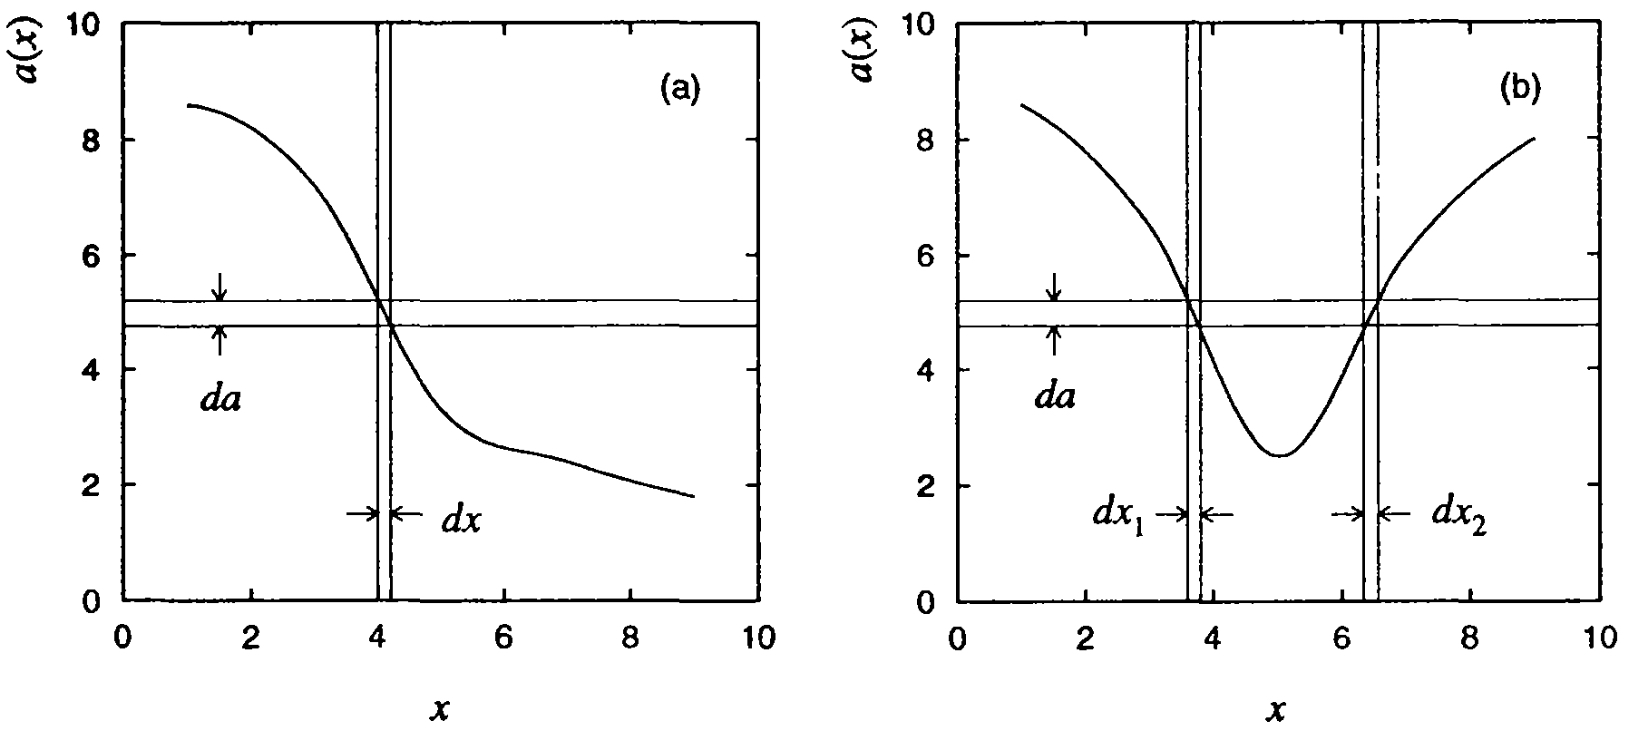
\includegraphics[width=0.99\textwidth,keepaspectratio]{figures/cowan/probability/RVfunc}
	\label{fig:RVfunc}
\end{figure}
\end{column}
\begin{column}{0.55\textwidth}
\begin{align*}
%&g(a)=f(x(a))|\TDy{a}{x}|\tag*{g(a)\,da=f(x)\,dx}\\
&g(a)\,da=|\int_{x(a)}^{x(a+da)}f(x')\,dx'|\\
&=\int_{x(a)}^{x(a)+|\TDy{a}{x}|da}f(x')\,dx'\Rightarrow g(a)=f(x(a))|\TDy{a}{x}|
\end{align*}
\end{column}
\end{columns}
%Distribuzione di probabilit\'a di $a(X)$ funzione di variabile casuale X con PDF $f(x)$:
\begin{align*}
&g(a')d\,a'=\int_{dS=\{a'\leq a(\vec{x})\leq a'+d\,a'\}}f(x_1,\ldots,x_n)d^n\,x,\ g(\vec{a})=f(\vec{x})/|\overset{\PDy{\vec{x}}{\vec{a}}}{J}|
\end{align*}
\begin{columns}[T]
\begin{column}{0.45\textwidth}
$\prob{(x)}=g(x)$, $\prob{(y)}=h(y)$, $z'=z'(x,y)$: $F_z(Z)=\int_Dp_{xy}(x,y)\,dx\,dy\ D=\{(x,y):z'(x,y)<z\}$
\begin{align*}
	&F_Z(a)=\prob{(Z=X+Y\leq a)}\\
	&=\iint_{X+Y\leq a}f_{XY}(x,y)\,dx\,dy\\
	&=\int_{X+Y\leq a}f_X(x)f_Y(y)\,dx\,dy\\
	&=\intsinf{}\int_{-\infty}^{a-y}f_X(x)\,dxf_Y(y)\,dy\\
	&=\intsinf{}F_X(a-y)f_Y(y)\,dy:\ f_Z(a)=\TDof{a}F_Z(a)
\end{align*}
\end{column}
\begin{column}{0.55\textwidth}
		\begin{columns}[T]
			\begin{column}{0.3\textwidth}
				\begin{figure}
					\centering
					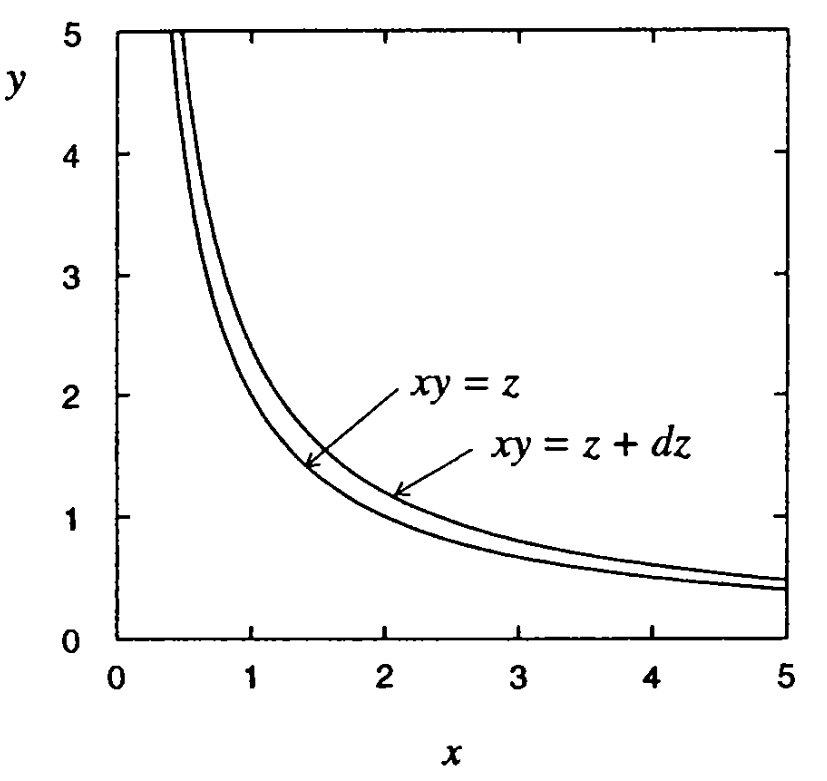
\includegraphics[keepaspectratio,width=0.9\textwidth]{figures/cowan/probability/RVprod}
					\label{fig:RVprod}
				\end{figure}
			\end{column}
			\begin{column}{0.7\textwidth}
				\begin{align*}
					&f(z)d\,z=\int_{d\,S}g(x)h(y)d\,xd\,y\\
					&=\intsinf{}g(x)d\,x\int_{\frac{z}{|x|}}^{\frac{z+d\,s}{|x|}}h(y)d\,y\\
					&f(z)=\intsinf{}g(\frac{z}{y})h(y)\frac{d\,y}{|y|}
				\end{align*}
			\end{column}
		\end{columns}
\end{column}
\end{columns}
\end{frame}

\begin{frame}{Somma di RV: Convoluzione e funzione caratteristica}
\begin{block}{Applicazione cambio di variabile}
Applicando regole cambio variabile per $Z=X+Y$ e $Y'=Y$ e marginalizzando su $Y'$ si trova: $f(Z=X+Y)=\intsinf{}f_X(Z-t)f_Y(t)\,dt$
\end{block}
\begin{block}{Antitrasformata di Fourier prodotto delle funzioni caratteristiche}
\begin{align*}
&X=X_1+X_2\\
&M_X(t)=M_{X_1}M_{X_2}
\end{align*}
La funzione caratteristica determina completamente pdf: se $F(X)$ continua, $dF(X)=f(X)dX$ allora $f(X)=\frac{1}{2\pi}\intsinf{}\phi_X(t)\exp{-iXt}\,dt$.
\end{block}
\begin{block}{Generate RV with given pdf: Inverse transform}
\begin{align*}
&x=\invers{F}(U)\\
&F_X(a)=\prob{(X<a)}=\prob{(\invers{F}(U\leq a))}=\prob{(U\leq F(a))}=F(a)
\end{align*}
\end{block}
\end{frame}

\section{Formule propagazione errori}

\begin{frame}{Formule propagazione errori}
\begin{block}{Teorema di Cramer}
$F(X,Y)$ continua,e derivataprima e seconda continua in intorno di $(M_x,M_y)$: RV $W=F(\bar{x},\bar{y})$ is asymptotically normal with $\E{[W]}=F(M_x,M_y)$,
\[\var{[W]}=[\PDy{X}{F}]_M^2\frac{\sigma^2_X}{n}+[\PDy{Y}{F}]_M^2\frac{\sigma^2_Y}{n}+2[\PDy{X}{F}]_M[\PDy{Y}{F}]_M\frac{\sigma_{XY}}{n}\]
\end{block}
\begin{block}{Error propagation}
\begin{align*}
&\E{[\hat{W}]}=\E{[F(\bar{x},\bar{y})]}\\
&=F(M_x,M_y)+\frac{1}{2}\{[\PtwoDy{X}{F}]\frac{\sigma_x^2}{n}+2[\PtwoMDy{X}{Y}{F}]\frac{\sigma_{xy}}{n}+[\PtwoDy{Y}{F}]\frac{\sigma_y^2}{n}\}\\
&\var{\hat{W}}=[\PDy{X}{F}]^2\frac{\sigma_x^2}{n}+[\PDy{Y}{F}]^2\frac{\sigma_y^2}{n}+2[\PDy{X}{F}][\PDy{Y}{F}]\frac{\sigma_{xy}}{n}
\end{align*}
\end{block}
\end{frame}

\begin{frame}{Estimators of population parameters}
\begin{align*}
&\bar{x}=\frac{1}{n}\sum_ix_i&M_x\tag{Mean: first moment}\\
&s_x^2=\frac{1}{n-1}\sum_i(x_i-\bar{x})^2&\sigma_x^2\tag{var: 2nd central moment}\\
&s_{xy}=\frac{1}{n-1}\sum_i(x_i-\bar{x})(y_i-\bar{x})&\sigma_{xy}\tag{covariance}\\
&r_{xy}=\frac{s_{xy}}{s_xs_y}&\rho_{xy}\tag{correlation coefficient}\\
&s_{\bar{x}}=\frac{1}{\sqrt{n}}s_x&\sigma_{\bar{x}}\tag{std deviation of average}\\
&v_x=\frac{s_x}{\bar{x}}&\frac{\sigma_x}{M_x}\tag{relative standard deviation}
\end{align*}
\end{frame}

\section{Funzione caratteristica/generatrice (dei momenti)}

\begin{frame}{Funzione generatrice dei momenti - Funzione caratteristica}
\begin{columns}[T]
	\begin{column}{0.4\textwidth}
		\begin{align*}
		&M_X(t)=\E{[\exp{tX}]}\\
		&\phi_X(t)=\E{[\exp{itX}]}=\int\exp{itx}\,d\mu_X(x)\\
		&\phi(0)=1,\ |\phi(t)|\leq1\\
		&Y=\alpha X+b:\ M_Y=\exp{ibt}M_X(\alpha t)\\
		&\mu_n(x_0)=\E{[\sum_k^n]}\binom{n}{k}(-1)^{n-k}\mu'_kx_0^{n-k}\\
		%&E[a(X)]=\intsinf{}a(x)f(x)dx=\intsinf{}ag(a)da
		\end{align*}
%	Non \'e detto che $f(\mu)=\E{[f]}$.
	\end{column}
	\begin{column}{0.6\textwidth}
		\begin{align*}
		&\PDyn{t}{M_X}{n}|_{t=0}=\E{[x^n]}=\mu_n'\\
		&\PDyn{(it)}{\phi_X}{n}|_{t=0}=(-i)^n\E{[x^n]}=\mu_n'\\
		&\phi_X(t)=\E{[\sum_r\frac{(itX)^r}{r!}]}\\
		&=\sum_r\frac{(it)^r}{r!}\E{[X^r]}=\sum_r\frac{(it)^r}{r!}\mu_r'\\
		&\phi_X(t)=1+i\mu t+\frac{1}{2}(\sigma^2+\mu^2)(it)^2
		\end{align*}
	\end{column}
\end{columns}
$\phi_X(t)$ determina completamente pdf: se $F(X)$ continua, $dF(X)=f(X)dX$ allora $f(X)=\frac{1}{2\pi}\intsinf{}\phi_X(t)\exp{-iXt}\,dt$
\begin{block}{Levy theorem: if sequenza $\phi_n\to\phi$ allora $X_n\xrightarrow{D}X$}
Per ogni RV con $\mu$ finita $\phi_X(t)\approx1+i\mu t+o(t)$,$\phi_{\frac{1}{n}X}(t)=\phi_X(\frac{t}{n})$, $\phi_{X+Y}(t)=\phi_X(t)\phi_Y(t)$:
$\phi_{\overline{X}_n}(t)=[\phi_X(t)]^n=[1+it\mu+\ldots]^n\to\exp{i\mu t}$
\end{block}
\end{frame}

\section{Legge grandi Numeri - T limite centrale}

\begin{frame}{Legge grandi numeri}
\begin{itemize}
\item Chebyshev ineq: $\prob{(|X-\mu|\geq k\sigma)}\leq\frac{1}{k^2}$
\item Probability convergence: 	Una sequenza di RV $\{X_n\}\to X$ in probabilit\'a se $\lim_{n\to\infty}\prob{(|X_n-X|)>\epsilon}$=0
\item LLN: $X_1,\ldots,X_n$ iid RV (RV campionata n volte): $\E{X_i}=\mu$, finite variance: $\var{X_i}=\sigma^2$ allora $\prob{(|\overline{X}_n-\mu|>\epsilon)}\leq\frac{\sigma^2}{n\epsilon^2}$, infatti
\begin{align*}
&\var{\overline{X}_n}=\var{\frac{1}{n}(X_1+\ldots+X_n)}\\
&=\frac{1}{n^2}\var{(X_1+\ldots+X_n)}=\frac{n\sigma^2}{n^2}=\frac{\sigma^2}{n}\\
&\prob{(|\overline{X}_n-\mu|>\epsilon)}\leq\frac{\sigma^2}{n\epsilon^2}
\end{align*}
\end{itemize}
\end{frame}

\begin{frame}{LLN: asintoticamente gaussiana - Teorema limite centrale (CLT)}
Se esistono $\mu_1, \mu_2$ finiti vale LLN: $\overline{x}_n-\mu\xrightarrow{P}0$.
\begin{columns}[T]
	\begin{column}{0.5\textwidth}
		\begin{align*}
		&\var{(\overline{x}_n-\mu)}=\var{(\frac{S_N}{N})}=\frac{1}{N^2}\var{(S_N)}=\frac{\sigma^2}{N}\\
		&\var{(S_N)}=\sum(\PDy{x_i}{S_N})^2\sigma_i^2
		%&\phi(t)=\phi_{X-\mu}
		\end{align*}
	\end{column}
	\begin{column}{0.5\textwidth}
		\begin{align*}
		&y_N=\sqrt{\frac{N}{\sigma^2}}(\overline{x}-\mu)\\
		&\E{[y_N]}=0,\ \var{[y_N]}=1\\
		&\phi_N=[\phi(\frac{t}{\sigma\sqrt{N}})]^N
		\end{align*}
	\end{column}
\end{columns}
\begin{align*}
&\phi(t)=\sum_{m=0}^{\infty}\left.\frac{d^m\phi}{dt^m}\right|_{t=0}\frac{t^m}{m!}=\sum_{m=0}^{\infty}\frac{(it)^m}{m!}\E{(y^m)}\approx1-\frac{t^2}{2N}\sigma^2-\frac{it^3}{3!}\frac{\E{[(x-\mu)^3]}}{n\expy{3/2}}+\ldots\\
&\log{\phi_N}=N\log{\phi(\frac{t}{\sigma\sqrt{N}})}\approx N[\frac{it\mu}{\sigma\sqrt{N}}+\frac{(it)^2\sigma^2}{2\sigma N}+o(\frac{t^3}{N\expy{\frac{3}{2}}})]\to-\frac{t^2}{2}\\
%\text{Per T Levy la pdf \'e:}\\
&\frac{1}{2\pi}\int\exp{-\frac{t^2}{2}}\exp{-itx}d\,t=\frac{1}{2\pi}\int\exp{(t+ix)^2-\frac{x^2}{2}}d\,t=\frac{1\exp{-\frac{x^2}{2}}}{\sqrt{2\pi}}
\end{align*}
\end{frame}

\begin{frame}[allowframebreaks]{PDFs}
Bernoulli: $\prob{(X=0)}=p$, $\prob{(X=1)}=q$, $\E{(X)}=p$, $\var{X}=p(1-p)$, $\phi_X(t)=\E[\exp{itX}]=p\exp{it}+q$.

Binomiale: k eventi con probabilit\'a p in sequenza di n estrazioni. Somma n variabili Bernoulli: $\prob{(k;n,p)}=\binom{n}{k}p^k(1-p)^{n-k}$, $\E{[k]}=\sum_kk\frac{N!}{k!(N-k)!}p^k(1-p)\expy{N-k}=Np$, $\mu'_q=\sum_k^nk^q\binom{n}{k}p^k(1-p)^{n-k}$, $\phi_X(t)=\E{[\exp{itX}]}=\sum_k\exp{itk}\binom{n}{k}p^k(1-p)^{n-k}=\phi_B^n(t)$; multinomiale: n trials with one success between k categories $f(x_1,\ldots,x_k;n,p_1,\ldots,p_k)=\frac{n!}{x_1!\ldots x_k!}p_1\expy{x_1}\ldots p_k\expy{x_k}$: $\sum x_i=n$, $\E{[X_i]}=Np_i\ \var{[X_i]}=Np_i(1-p_i)$, CF: $(\sum_j^kp_j\exp{it_j})^n$.

Poissoniane! $\prob{(k;\mu)}=\frac{\mu^k}{k!}\exp{-\mu}$, $\E{[k]}=\sum_{k=0}^{\infty}k\frac{\mu^k}{k!}\exp{-\mu}$, $\E{[k^2]}=\sum_{k=0}^{\infty}k^2\frac{\mu^k}{k!}\exp{-\mu}=\mu^2+\mu$, $\var[k]=\E{[k^2]}-(\E{[k]})^2=\mu$, $M_P(t)=\sum_k\exp{tk}\frac{\mu^k}{k!}\exp{-\mu}=\Exp{\mu(\exp{t}-1)}$.

Esponenziale: $p(t;\lambda)=\lambda\exp{-\lambda t}$, $p(t;\xi)=\frac{1}{\xi}\exp{-\frac{t}{\xi}}$, $\phi_e(t)=\frac{1}{1-it\xi}$, $M_e(t)=\lambda\intzi{}\exp{-(\lambda-t)x}\,dx=\frac{\lambda}{\lambda-t}$.

Uniforme: $f(x;\alpha,\beta)=\left\{\begin{array}{c}\frac{1}{\beta-\alpha}\\0\\
			\end{array}\right.$, $\var{[x]}=\frac{1}{12}m^2$, $\phi_U=\frac{\exp{i\beta t}-\exp{i\alpha t}}{(\beta-\alpha)it}$
\end{frame}

\begin{frame}{Propriet\'a $\chi^2$}
La distribuzione di chi-squared con $\nu$ gradi di libert\'a $\prob{(\chi_{\nu}^2)}$ \'e la distribuzione di probabilit\'a di $\sum_1^{\nu}x_i^2$ con $x_i\to N(0,1)$ ($\sum_{i=1}^N\frac{(x_i-\mu_i)^2}{\sigma_i^2}$), $\chi^2$ non centrale $x_i\to N(\mu_i,1)$, parametro non centralit\'a $\lambda=\sum\mu_i^2$.
\begin{columns}[T]
	\begin{column}{0.7\textwidth}
		Funzione caratteristica: $y=\frac{(x_i-\mu_i)}{\sigma_i}$, $z=y^2$
		\begin{align*}
		&f(z;n=1)=2\phi(y)|\TDy{z}{y}|=\frac{1}{\sqrt{2\pi z}}\exp{-z/2}\\
		&\phi_1(t)=\E_z{(\exp{itz})}=(1-2it)\expy{-1/2}\\
		%&=\intsinf{}\frac{\exp{itx-x^2/2}}{\sqrt{2\pi}}\,dx=\frac{1}{\sqrt{1-2it}},\\
		&\phi_{\chi^2_{\nu}}(t)=(1-2it)\expy{-\frac{\nu}{2}}
		\end{align*}
	\end{column}
	\begin{column}{0.3\textwidth}
		\begin{align*}
		&\E{(\chi^2_{\nu})}=\nu\\
		&\var{[\chi_{\nu}^2]}=2\nu\\
		&\E{(\chi^{2,NC}_{\nu})}=\nu+\lambda
		\end{align*}
	\end{column}
\end{columns}
\begin{align*}
&\prob{(x=\chi^2_{\nu})}=\frac{1}{2\expy{\nu/2}\Gamma(\frac{\nu}{2})}x\expy{\frac{\nu}{2}-1}\exp{-\frac{x^2}{2}}\xrightarrow{\nu\to\infty}N(\nu,2\nu)
\end{align*}
Approssimazione di Fisher: $\prob{(\sqrt{2\chi^2})}\approx N(\sqrt{2\nu-1},1)$
\end{frame}

\section{Data analysis}

\begin{frame}{Inference's tools}
\begin{itemize}
\item Likelihood $L_{x_0}(m)=p(x_0;m)$, se x,y eventi indipendenti: $L_{(x_0,y_0)}(m)=L_{x_0}(m)L_{y_0}(m)$, Ripetendo gli esperimenti la likelihood diventa pi\'u piccata.
\item Definita a meno di costante moltiplicativa ($\log{L}$): invariante per cambiamento di osservabile (funzione solo dei dati)
$L_{f(t_0)}(m)=|J(t_0)|L_{t_0}(m)$
\item Bayes theorem and Likelihood - Posterior ratio (Degree of belief): $\frac{\Pi(\theta_1|x_0)}{\Pi(\theta_2|x_0)}=\frac{L_{x_0}(\theta_2)}{L_{x_0}(\theta_1)}\frac{\Pi(\theta_2)}{\Pi(\theta_1)}$.
\end{itemize}
\end{frame}

\begin{frame}{Esempi di likelihood}
\begin{columns}[T]
\begin{column}{0.3\textwidth}
\begin{itemize}
\item Bernoulli:
\begin{align*}
&L_0=1-p\\
&L_1=p
\end{align*}
\item L per $U(0,m)$:
\[\frac{1}{m}:\ x<m\]
\end{itemize}
\end{column}
\begin{column}{0.7\textwidth}
\begin{itemize}
\item N RV iid con pdf esponenziale
\begin{align*}
&\prob{(t,\tau)}=\frac{1}{\tau}\exp{-\frac{t}{\tau}}\\
&L_{(t_1,\ldots,t_n)}(\tau)=\prod_i^n\frac{1}{\tau}\exp{-\frac{t_i}{\tau}}\\
&=\frac{1}{\tau^n}\exp{-\frac{\sum t_i}{\tau}}=\frac{1}{\tau^n}\exp{-\frac{n\overline{t}}{\tau}}
\end{align*}
\end{itemize}
\end{column}
\end{columns}
\end{frame}

\begin{frame}{Statistica}
		\begin{block}{Momenti di una statistica S}
	\begin{align*}
	&\E{[(S(\vec{x})-\E{[S]})^l]}
	\end{align*}
\end{block}
\begin{block}{Propagazione errori}
\begin{align*}
&S(\vec{x})\approx y(\vec{\mu})+\left.\sum_i^n\PDy{x_i}{S}\right|_{\vec{\mu}}(x_i-\mu_i)+o(|\vec{x}-\vec{\mu}|)\\
&\var{(S)}=\E{[(S(\vec{x})-\E{[S]})^2]}\approx\sum_{ij}\PDyat{x_i}{S}{\vec{\mu}}\PDyat{x_i}{y}{\vec{\mu}}\cov{x_ix_j}\\
&\cov{x_ix_j}=\E{[(x-\mu_x)(y-\mu_y)]}=\E{[xy]}-\mu_x\mu_y
\end{align*}
\end{block}
\begin{block}{Statistica sufficiente}
Statistica sufficiente $S$ per parametro $\Theta$. Pdf di X data $T(X)$ non dipende da parametro $\theta$: $\prob{(x;S,\theta)}=\prob{(x;S)}$.
Statistica sufficiente minimale
	$S$ sufficiente e esiste una funzione $f$ per ogni $s_i$ con $S=f(s_i)$ e $\dim({S})\leq\dim{(X)}$.
\end{block}
\end{frame}

\begin{frame}{Statistiche sufficienti per il parametro dato. T di Darmois}
\begin{block}{Teorema di fattorizzazione}
	Probabilit\'a di osservare $X$ dato $\theta$ \'e probabilit\'a di $S(x)$ dato $\theta$ per funzione sole osservabili: $\prob{(x;\theta)}=\prob{(S(x);\theta)}h(x)$ e $\omega_{\theta}$ non dipende da $\theta$
\end{block}
\begin{block}{Teorema di Darmois: condizione necessaria e sufficiente per esistenza statistica sufficiente}
	Esiste S tale che $\dim{(S)}<\dim{(X)}$ iff
	\begin{align*}
	&p(\vec{x}|\theta)=\Exp{[\sum_i^n\alpha_i(\vec{x})a_i(\theta)+\beta(\vec{x})+\gamma(\theta)}\\
	&S_j=\sum_i\alpha_j(x_i)
	\end{align*}
	Esiste statistica suff. iff: supporto pdf non dipende da parametro e appartiene alla famiglia esponenziale.
\end{block}
\end{frame}

\begin{frame}[allowframebreaks,fragile]{Dimostrazioni S sufficiente}
n RV iid con pdf bernoulli p:
	$X_1,\ldots,X_n$: iid con pdf di Bernoulli, supporto pdf $\chi=\{0,1\}$, parametro p nell'intervallo $(0,1)$:
	\begin{align*}
	&T=\sum X_i\to\{0,\ldots,n\}&\intu{con pdf binomiale}
	&\prob{(X_1=x_1\cap\ldots X_n=x_n|T=t)}=0, t\neq\sum x_i\\
	&=\prob{(\cap_iX_i=x_i|T=t)}=\frac{\prob{((\cap_iX_i=x_i)\cap(T=t))}}{\prob{(T=t)}}=\frac{\prob{(\cap_iX_i=x_i)}}{\prob{(T=t)}}\intu{se $\sum x_i=t$:}
	&A=\{\cap_iX_i=x_i\}\subseteq B=\{T=t\}
	\end{align*}
	e poich\'e le $X_i$ sono indipendenti si ha
	\begin{align*}
	&\frac{\prod\prob{(X_i=x_i)}}{\prob{(T=t)}}=\frac{p^{\sum x_i}(1-p)^{n-\sum x_i}}{\binom{n}{t}p^t(1-p)^{n-t}}
	\end{align*}

n RV iid Poisson$(\lambda)$:
	$X_1,\ldots,X_n$: iid con pdf di Poisson con parametro ignoto $\lambda$:
	\begin{align*}
	&\prob{(X_1=x_1\cap\ldots X_n=x_n|T=t)}=\prob{(\cap_iX_i=x_i|T=t)}\\
	&\frac{\prob{((\cap_iX_i=x_i)\cap(T=t))}}{\prob{(T=t)}}=\frac{\prob{(\cap_iX_i=x_i)}}{\prob{(T=t)}},\ t=\sum x_i\\
	&=\frac{\prod_i[\frac{\exp{-\lambda}\lambda^{x_i}}{x_i!}]}{\frac{\exp{-\lambda}(n\lambda)^t}{t!}}=\frac{t!}{\prod x_i!}n^{-t}
	\end{align*}

%Gaussiana: media ignota, varianza nota:
%	\begin{align*}
%	&L(\overline{x};\mu)=\prod_iL(x_i;\mu,\sigma)=(\frac{1}{\sqrt{2\pi}\sigma})^N\underbrace{\exp{-\frac{N}{2}\frac{\sum_i(\overline{x}-\mu)^2}{\sigma^2}}}_{g(T,\theta)}\underbrace{\exp{-\frac{N}{2}\frac{\sum_i(x_i-\overline{x})^2}{\sigma^2}}}_{h(\vec{x})}
%	\end{align*}
%	La statistica ''media aritmetica'' \'e sufficiente per parametro $\mu$ della gaussiana (dominio gaussiana non dipende da $\mu$) (Ex: pdf della media aritmetica)
%Gaussiana: media nota, varianza ignota:
%	$\hat{\sigma}^2=\frac{\sum x_i^2-\mu}{N}$ \'e sufficiente per $\sigma^2$ (pdf di $\hat{\sigma}^2\propto g$ e dominio gaussiana non dipende da $\sigma$). (Ex: statistica sufficiente $\sigma$ gaussiana)
%Media aritmetica \'e statistica sufficiente per parametro binomiale, poissoniana, esponenziale:
%	\begin{align*}
%	&\prob{(k)}=\binom{n}{k}p^k(1-p)^{n-k}\\
%	&\prob{(k)}=\frac{\mu^k\exp{-\mu}}{k!}\\
%	&\prob{(x)}=\lambda\exp{-\lambda x}
%	\end{align*}

Distribuzione uniforme: $x_{max}$ statistica sufficiente:
\begin{align*}
&\prob{(x;m)}=\left\{\begin{matrix}\frac{1}{m}\ x\in[0,m]\\0\\\end{matrix}\right.&\intertext{estraggo N $x_1,\ldots,x_n$}\\
&L(\vec{x},m)=\prod_iL(x_i;m)=\left\{\begin{matrix}\frac{1}{m^N}\ m>x_{max}\\0\ m<x_{max}\\\end{matrix}\right.
\end{align*}
%$g(T,\theta)\propto A(T;\theta)$ dove $A$ \'e pdf di statistica $T$?
\begin{align*}
&\prob{(x_{max}<x_0)}=F_M(x_0)=\prod_i\prob{(x_i<x_0)}=\prod_i\int_0^{x_0}\frac{1}{m}\,dx=(\frac{x_0}{m})^N\\
&\prob{(x_M;m)}=\TDof{x_0}\left.F_M(x_0)\right|_{x_M}=\frac{N}{m}(\frac{x_M}{m})^{N-1}I(x_M<m)\\
&L_{\vec{x}}(m)=\frac{N}{m^N}x_M^{N-1}\frac{1}{Nx_M^{N-1}}=\prob{(x_M;m)}\frac{1}{Nx_M^{N-1}}\ m>x_M
\end{align*}
$\prob{(x;S,\theta)}=\prob{x;S}$!
Media aritmetica \'e statistica sufficiente per parametro binomiale, poissoniana, esponenziale: $\log{\binom{n}{k}}+k\log{\frac{p}{1-p}}+n\log{(1-p)}$: $S=\sum_ik_i$, $k\log{\mu}-\mu-\log{k!}$: $S=\sum_ik_i$, $-\lambda x-\mu+\log{\lambda}$: $S=\sum_ix_i$.
Gaussiana media ignota:
	\begin{align*}
	&L(\overline{x};\mu)=\prod_iL(x_i;\mu,\sigma)=(\frac{1}{\sqrt{2\pi}\sigma})^N\exp{-\frac{N}{2}\frac{\sum_i(\overline{x}-\mu)^2}{\sigma^2}}\exp{-\frac{N}{2}\frac{\sum_i(x_i-\overline{x})^2}{\sigma^2}}\\
	&\alpha(x)=x\ \Rightarrow\ T=\frac{1}{N}\sum x_i=\exv{X}
	\end{align*}
Gaussiana varianza ignota:
	\begin{align*}
	&L(\overline{x};\mu)=\prod_iL(x_i;\mu,\sigma)=(\frac{1}{\sqrt{2\pi}\sigma})^N\exp{-\frac{N}{2}\frac{\sum_i(\overline{x}-\mu)^2}{\sigma^2}}\exp{-\frac{N}{2}\frac{\sum_i(x_i-\overline{x})^2}{\sigma^2}}\\
	&\alpha(x)=x\mu-\frac{x^2}{2}:\ T=\sum(x_i\mu-\frac{x_i^2}{2})\\
	&\hat{\sigma}^2=\frac{\sum(x_i-\mu)^2}{N}=\frac{N\mu^2-2T}{N}
	\end{align*}
Spazio dei parametri della Gaussiana:
	\begin{align*}
	&\log{\prob{(\vec{x};\mu,\sigma^2)}}=-\log{(\sqrt{2\pi}\sigma)}-\frac{x^2}{2\sigma^2}+\frac{x\mu}{2\sigma^2}+\frac{\mu^2}{2\sigma^2}\\
	&\alpha_1(x)=x,\ a_1(\mu)=\mu,\ \alpha_2(x)=-\frac{x^2}{2},\ a_2(\sigma^2)=\frac{1}{\sigma^2},\ S_{\mu}=\sum x_i\\
	&S_{\sigma^2}=-\sum\frac{x_i^2}{2}
	\end{align*}
\end{frame}

\section{Stima puntuale}

\begin{frame}{Propriet\'a generali stiamatori}
Statistica $\hat{\Theta}(X_1,\ldots,X_n)$ che fornisce stima di funzione dei parametri $\tau(\Theta)$
\begin{itemize}
	\item Consistenza (LGN): $\prob{\hat{\theta}}\to\theta_0$
	\item Varianza $\var{\vec{X}}\to\frac{1}{N}$ - Bias $b(\vec{x})$ non diminuisce all'aumentare delle misure; scuola soggettivista: bias non esiste.
	\item distribuzione semplice
\end{itemize}
\begin{columns}[T]
	\begin{column}{0.45\textwidth}
	Riduzione del bias:
		\begin{align*}
	&\E{[S(x)]}=\theta+b(\theta)\\
	&\to\ S'(x)=S(x)-b(\hat{\theta})-\hat{b}(x)\\
	&\E{[\hat{b}(x)]}=b(\hat{\theta})\\
	&\var{[S']}=\var{[S]}+\var{[b]}
	\end{align*}
	Metodo empirico
	\begin{align*}
	&S_N'(x)=2S_N(x)\\
	&-\frac{1}{2}[S_{\frac{N}{2}}(x_1,\ldots,x_{\frac{N}{2}})+S_{\frac{N}{2}}(x_{\frac{N}{2}},\ldots,x_N)]
	\end{align*}
	\end{column}
	\begin{column}{0.55\textwidth}
		\begin{itemize}
			\item unbiased estimator: $\E_{\Theta}[T]=\tau(\Theta)$
			\item estimator bias: $B_{\Theta}(T)=\E_{\Theta}[T]-\tau(\Theta)$
			\item Estimator mean square error: $\E{[(T-\tau(\Theta))^2]}=V_{\Theta}[T]+(\E{[T]}-\tau(\Theta))^2$
			\item Stimatori consistenti: $\lim_{n\to\infty}T_n(X_1,\ldots,X_n)\overset{P}{=}\tau(\Theta)$
		\end{itemize}
	\end{column}
\end{columns}
\end{frame}

\begin{frame}{Informazione di Fischer}
	Informazione contenuta nei dati su un parametro $\Theta$: la condizione di massimo su log L da lo stimatore, la curvatura determina la massima precisione dello stimatore
	\begin{align*}
	&\overbrace{I_X(\Theta)}^{\text{n RV iid:}=nI_{X_1}}=\E_{\Theta}{[(\PDof{\Theta}\log{f(X;\Theta}))^2]}=\overbrace{-\E_{\Theta}{[\PtwoDof{\Theta}\log{f(X;\Theta)}]}}^{\text{se esistono finiti $\PtwoDof{\Theta}$ e $\E{}$}}
	\end{align*}
	Per due parametri:
	\begin{align*}
	&I_X(\Theta)=\begin{pmatrix}I_{11}(\Theta)&I_{12}(\Theta)\\I_{21}(\Theta)&I_{22}(\Theta)\end{pmatrix}\ I_{ij}(\Theta)=-\E{[\frac{\partial^2}{\partial\Theta_i\partial\Theta_j}\log{f(X;\Theta)}]}
	\end{align*}
	\begin{block}{Score statistics}
		\begin{columns}[T]\begin{column}{0.5\textwidth}
				
			\end{column}\begin{column}{0.5\textwidth}
				$I_X(\Theta)\geq I_T(\Theta)$: l'uguaglianza vale iff T \'e sufficiente per $\Theta$.
		\end{column}\end{columns}
	\end{block}
\end{frame}

\begin{wordonframe}{Esempi Informazione}
	Poisson: $I_X(\lambda)=\invers{\lambda}$;
	Gaussian: $I_X(\mu)=\sigma\expy{-2}$;
	N RV iid: $I_X(\Theta)=nI_{X_1}(\Theta)$;
	N RV gaussiane $N(\mu,\sigma^2)$: matrice informazione
	$\vec{X}=(X_1,\ldots,X_n)$ e $\vec{\Theta}=(\mu,\sigma^2)$
	\begin{align*}
	&I_{11}=\E{[(\PDof{\mu}\log{f})^2]}=\sigma\expy{-2}\ I_{22}=\E{[(\PDof{\sigma^2}\log{f})^2]}=\frac{1}{2}\sigma\expy{-4}\\
	&I_{12}=I_{21}=\frac{1}{2\sigma^2}\E{[\sigma\expy{-3}(X_1-\mu)^3-(X_1-\mu)]}=0
	\end{align*}
\end{wordonframe}

\begin{frame}{Best unbiased estimator: Disuguaglianza di Cramer-Rao (CRLB)}
$X_1,\ldots,X_n$ iid con pdf $f(x,\Theta)$: se supporto $\Omega_{\Theta}$ di $f(x,\Theta)$ non dipende da $\Theta$ e integrali in $dx$ sono invertibili con $\PDof{\Theta}$; esiste stimatore unbiased $T(\vec{X})\xrightarrow{\E{[\ ]}}\tau(\Theta)$ con $\PDy{\Theta}{\tau}$ esiste finito, allora:
\begin{align*}
&V_{\Theta}[T]\geq\frac{[\tau'(\Theta)]^2}{n\E_{\Theta}[(\PDof{\Theta}\log{f(X_1;\Theta)})^2]}=\frac{[\tau'(\Theta)]^2}{nI_{X_1}(\Theta)}\\
&\left(\frac{(1+\TDy{\theta}{b})^2}{I_{\hat{\Theta}}(\theta)}\right)
\end{align*}
minimum variance bound
\end{frame}

\section{Costruzione stimatori consistenti}

\begin{frame}{Logica stimatori consistenti - Stimatori impliciti}
\begin{align*}
&\xi(\theta)=\invers{N}\sum_ia(X_i,\theta)\xrightarrow{N\to\infty}\E{[a(X,\theta)]}=\int a(X,\theta)f(X;\theta)\,dX=h(\theta)
\end{align*}
\hypo{$a$ ha varianza finita}, \hypo{$h(\theta_0)=0$}: per LLN uno zero di $\xi(\theta)$ converge a $\theta_0$, $\xi(\hat{\theta})=0$ \keyword{stimatore implicito}.
\begin{columns}[T]
\begin{column}{0.6\textwidth}
One of the root of $h(\theta)$ give consistent estimate of $\theta_0$ if $\xi$ is differentiable, mean of $\xi$, $\PDy{\theta}{\xi}$ exist and $\lim_{N\to\infty}\E{[\PDy{\theta}{\xi(\theta)}]_{\theta=\theta_0}}\neq0$.
\end{column}
\begin{column}{0.4\textwidth}
\begin{figure}
	\centering
	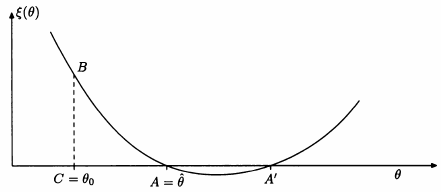
\includegraphics[width=0.99\textwidth,keepaspectratio]{figures/james/estimators/estimpl}
	\label{fig:estimpl}
\end{figure}
\end{column}
\end{columns}

In practice one find $a(X,\theta)$ extremizing other function g: $a(X_i,\theta)=\PDof{\theta}g(X_i,\theta)$: a root of $\xi{\theta}=\invers{N}\sum_i^Ng(X_i,\theta)=0$ is C-estimator of $\theta_0$: hp are meet if
\begin{align*}
&a(X_i,\theta_0)=\PDy{\theta}{[g(X_i,\theta)-\E{[g(X_i,\theta)]}]}|_{\theta_0},\ \E{(a(X_i,\theta_0))}=0
\end{align*}
and $\E{\PDy{\theta}{g(X_i,\theta)}}$ don't depends on $\theta_0$.
\end{frame}

\begin{frame}{Moment method as implicit estimator}
\begin{align*}
&a(X_i,\theta)\to a(X_i)-\E{[a(X)]}, g(X_i,\theta)=a(X_i)\theta-\int_{\theta_0}^{\theta}\int a(X)f(X,\theta)\,dX\,d\theta
\end{align*}
Ho N osservazioni $x_1,\ldots,x_n$ di RV iid con pdf $f(x,\theta)$, $\theta=(\theta_1,\ldots,\theta_m)$. Cerco m funzioni linindip $a_i(X)$ quindi il valore di aspettazione dipende dal valore vero del parametro:
\begin{align*}
&\E{[a_k(X)]}=\int a_k(x)f(x;\theta)\,dx=e_k(\theta):\ \E{[X^k]}=\frac{\sum_i\E{[x_i^k]}}{N}\xrightarrow{P}\mu'_k\\
&\hat{\theta}=\invers{e}[\invers{N}\sum_i^Na(X_i)]
\end{align*}

\begin{columns}[T]
\begin{column}{0.65\textwidth}
	\begin{align*}
	&\cov{(x_i,x_j)}=\E{[x_ix_j]-\E{[x_i]}\E{[x_j]}}\\
	&=\frac{\mu'_{i+j}-\mu_i'\mu_j'}{N}\\
	&\cov{[\hat{\theta}_i,\hat{\theta}_j]}=\sum_{k,l}\PDy{\hat{e}_k}{\hat{\theta}_i}\PDy{\hat{e}_l}{\hat{\theta}_j}\cov{[\hat{e}_k,\hat{e}_l]}
	\end{align*}
	Co-var matrix of estimators (error propagation formula)
\end{column}
\begin{column}{0.35\textwidth}
	\begin{align*}
	&m_1=\mu_1'(\theta_1,\ldots,\theta_n)\\
	&\vdots\\
	&m_n=\mu_n'(\theta_1,\ldots,\theta_n)\intd{Invertendo il sistema sopra si trovano gli stimatori:}
	&\hat{\theta_1}(m_1,\ldots,m_m)\\
	&\vdots\\
	&\hat{\theta_m}(m_1,\ldots,m_m)
	\end{align*}
\end{column}
\end{columns}
\end{frame}

\begin{wordonframe}{Examples moment estimators}
\begin{columns}[T]\begin{column}{0.5\textwidth}
	\begin{block}{Uniforme $U(a,b)$}
		\begin{align*}
		&\mu_1=\E{[X]}=\frac{1}{2}(a+b)\\
		&\mu_2=\E{[X^2]}=\frac{1}{3}(a^2+ab+b^2)\\
		&\hat{a}=\mu_1\pm\sqrt{3(\mu_2-\mu_1^2)}\\
		&\hat{b}=2\mu_1-a
		\end{align*}
	\end{block}
\end{column}\begin{column}{0.5\textwidth}
	
\end{column}\end{columns}
\end{wordonframe}

\begin{frame}{Stimatori di massima likelihood (as stimatori impliciti)}
\begin{align*}
&a(X,\theta)=\PDy{\theta}{\log{L}}=\PDof{\theta}g(X_i,\theta)\\ %&K_N=\xi=\frac{1}{N}\PDof{\theta}\sum_i^Ng(X_i,\theta)=\frac{1}{N}\sum_i\PDy{\theta}{\log{(L(x_i,\theta))}}=0\tag{}\\
&K_N=\xi=\frac{1}{N}\PDof{\theta}\sum_i^Ng(X_i,\theta)\PDof{\theta}\sum_i^N\ln{f(X_i,\theta)}=\PDof{\theta}\ln{L(\vec{X},\theta)}=0 \tag*{(Likelihood equation)}\\
%&K_N=\frac{1}{N}\PDof{\theta}\sum_i^Ng(X_i,\theta)=0:\\
&\E{[\PDy{\theta}{\xi}|_{\theta_0}]}=\E{[\frac{1}{N}\PtwoDy{\theta}{\ln{L(\vec{X},\theta)}}|_{\theta_0}]}\xrightarrow{N\to\infty}\E{[\PtwoDy{\theta}{\ln{f(X,\theta)}}|_{\theta_0}]}\\
&\E{[\PDy{\theta}{K}]}=\E{[\PtwoDy{\theta}{\log{L}}]}=-\E{[(\PDy{\theta}{\ln{f(X,\theta)}})^2]}=-I_X<0
\end{align*}
so the root $\hat{\theta}$ correspond to maximum of L. The quantity $\PDof{\theta}\ln{L(\vec{X},\theta)}$ \'e asintoticamente gaussiano con media 0 e varianza $NI(\theta)$
\end{frame}

\begin{frame}[allowframebreaks]{Propriet\'a MLE}
\begin{block}{Consistente se soluzione della likelihood equation \'e unica: massimo assoluto (asintotico) \'e consistente}
$\PDy{\theta}{\log{L_{tot}}}=0$.
\end{block}
\begin{block}{Invariante per trasformazione di parametro}
$\tau(\lambda)=\frac{1}{\lambda}$: $\hat{\tau}=\frac{1}{\hat{\lambda}}$
\end{block}
\begin{block}{Asintoticamente un-biased}
\end{block}
\begin{block}{Asintoticamente efficente: $\var{[\hat{\theta}]}\to\frac{1}{NI_{X_1}}$}
\begin{align*}
&K_N(\hat{\theta)}=K(\theta_0)+\PDy{\theta}{K_N}(\hat{\theta}-\theta_0)+o(\hat{\theta}-\theta_0)^2\intd{prendendo il valore di aspettazione}
&0=\sum_i\frac{\PDy{\theta}{\log{(L(x_i))}}}{N}-I(\hat{\theta}-\theta_0)+(\var{[\hat{\theta}]})\\
&\hat{\theta}-\theta_0\propto N(0,\frac{1}{NI})+\frac{\const{}}{N}: \lim_{N\to\infty}b(\hat{\theta})\propto\frac{1}{N}
\end{align*}
\end{block}
\begin{block}{Pdf dello stimatore tende asintoticamente ad gaussiana}
\end{block}
\begin{block}{\keyword{MLE per pdf esponenziale}}
Per pdf esponenziale\[f(x;\theta)=\exp{\alpha(x)a(\theta)+\beta(x)+c(\theta)}\] il metodo di massima likelihood determina lo stimatore efficiente e senza bias $\hat{M}=\frac{1}{N}\sum_i\alpha(x_i)$ di $M(\theta)=-\frac{\TDy{\theta}{c(\theta)}}{\TDy{\theta}{a(\theta)}}$.
\end{block}
\end{frame}

\begin{wordonframe}{MLE in pratica}
\begin{block}{binning}
\begin{columns}[T]
\begin{column}{0.5\textwidth}
N fissato
\begin{align*}
&\prob{(\vec{k},\theta)}=\frac{N!}{\prod_ik_i!}\prod_i{\underbrace{\prob{(i)}}_{\int_{S_i}\prob{(x|\theta)}\,dx}}\mkern-20mu^{k_i}\\
&\max{[\sum_i k_i\log{[\prob{(x;\theta)}\Delta]}]}\\
&\to\max{[\sum_i \log{[\prob{(n_i;\theta)}]}]}
\end{align*}
\end{column}
\begin{column}{0.5\textwidth}
N variabile: Extended likelihood, normalizzazione varia
\begin{align*}
&\mu_i=\mu_TP_i(\theta)\\
&\prob{(k_i\theta)}=\frac{\prod_i\exp{-\mu_TP_i}(\mu_TP_i)^{k_i}}{k_i!}\\
&\log{L}=\sum_ik_i\log{P_i(\theta)}+k_i\log{\mu_T}\\
&-\mu_TP_i-\bcancel{\log{k!}}\\
&\left\{\begin{matrix}\mkern-240mu\PDy{\theta_i}{\log{L}}=0\\\PDy{\mu_T}{\log{L}}=0\ (:L(\bcancel{\mu_T}),\mu_T(\bcancel{\theta_i}) \Rightarrow\ \mu_T=N)\\\end{matrix}\right.
\end{align*}
\end{column}
\end{columns}
\end{block}

\begin{block}{Fit resolution of histogram (??)}
$A=\sum_i\frac{1}{P_i}(\PDy{\theta}{P_i})^2$
\end{block}\end{wordonframe}

\begin{frame}[allowframebreaks]{Esempi di stimatori di massima likelihood}
Binomiale: $K_1,\ldots,K_N:\ f(k;n,p)=\binom{n}{p}p^k(1-p)^{n-k}$
\begin{align*}
&\log{(L(\vec{k},p))}=\log{[\prod_i^N\binom{n}{k_i}p^{k_i}(1-p)^{n-k_i}]}\\
&\max{(L)}:\ \TDof{p}\log{(L)}=\sum_i^N[\frac{k_i}{p}+(n-k_i)\frac{(-1)}{1-p}]=0\Rightarrow\sum^Nk_i=Nnp\\
&\hat{p}_{MLE}=\sum\frac{k_i}{Nn}=\exv{k}\\
&\E{[\hat{p}]}=\frac{1}{N}\frac{\sum\E{[k_i]}}{n}=\frac{\sum^Npn}{nN}=p\\
&\var{[\hat{p}]}=\var{[\frac{1}{nN}\sum k_i]}=\frac{1}{n^2N^2}Nnp(1-p)\\
&I_{k_i}(p)=\frac{nN}{p(1-p)}\to\frac{1}{\var{}}: MVB
\end{align*}

Gaussiana:
Ho N misure $x_i$ da RV con distro gaussiana: cerco MLE per $\mu, \sigma^2$.
\begin{columns}[T]
\begin{column}{0.5\textwidth}
\begin{align*}
&G(x;\mu,\sigma)=\frac{1}{\sqrt{2\pi\sigma^2}}\exp{-\frac{(x-\mu)^2}{2\sigma^2}}\\
&\log{L}=-N\log{\sigma}-\frac{1}{2\sigma^2}\sum_i^N(x_i-\mu)^2\\
&\E{[\hat{\sigma^2}]}=\frac{1}{N}\sum_i\E{[x_i^2-2x_i\exv{x}+\exv{x}^2]}\\
&\E{[x_i^2]}=\mu^2+\sigma^2\\
&\E{[x_i\exv{x}]}=\frac{1}{N}\E{[x_i^2+\sum_{j\neq i}x_ix_j]}\\
&\E{[\exv{x}^2]}=\E{\frac{\sum x_i\sum x_j}{N^2}}=\mu^2+\frac{\sigma^2}{N}
\end{align*}
\end{column}
\begin{column}{0.5\textwidth}
Maximum of $\log{L}$ for $\mu, \sigma^2$
\begin{align*}
&\PDy{\mu}{\log{L}}=0\\
&\hat{\mu}=\frac{\sum x_i}{N}\\
&\PDy{\sigma}{\log{L}}=0\\
&-\frac{N}{\sigma^2}+\frac{1}{\sigma^4}\sum^N(x_i-\exv{x}(\to\mu))=0\\
&\hat{\sigma^2}=\frac{\sum(x_i-\exv{x})^2}{N}\intd{T darmois in 2D: stat. suff.:}
&\sum x_i,\ \sum x_i^2
\end{align*}
\end{column}
\end{columns}
$\E{[\hat{\sigma^2}]}=\frac{N-1}{N}\sigma^2$ quindi definisco lo stimatore unbiassato $\hat{\sigma^2}'=\frac{\sum(x_i-\exv{x})^2}{N-1}$.

\begin{columns}[T]
\begin{column}{0.6\textwidth}
Esponenziale: cambio di parametro. $p(x;\tau)=\frac{1}{\tau}\exp{-\frac{x}{\tau}}=\lambda\exp{-\lambda x}=p(x;\lambda)$:
\end{column}
\begin{column}{0.4\textwidth}
likelihood \'e invariante per cambio di parametro
\end{column}
\end{columns}
\begin{columns}[b]
\begin{column}{0.4\textwidth}
$\hat{\tau}_{MLE}=\frac{\sum_ix_i}{N}:\ \E{[\hat{\tau}]}=\tau,\ I_x(\tau)=\frac{1}{\var{\hat{\tau}}},\ \var{\hat{\tau}}=\frac{\tau^2}{N}$
\end{column}
\begin{column}{0.6\textwidth}
$\log{L}=N\log{\lambda}-\lambda\sum_ix_i$, $\TDy{\lambda}{\log{\lambda}}=0$. $\hat{\lambda}=\frac{N}{\sum x_i}=\frac{1}{\hat{\tau}}$, $\E{[\hat{\lambda}]}=\frac{N}{N-1}\lambda$
\end{column}
\end{columns}
\begin{align*}
&\phi_x(k)=\E{[\exp{ikx}]}=\intzi\exp{ikx}\exp{-\lambda x}\lambda\,dx=\frac{1}{1-i\frac{k}{\lambda}}\\
&\phi_{\sum x_i}\frac{1}{(1-\frac{ik}{\lambda})^N},\ z=\sum x_i\ \text{distribuzione di Erlang}\downarrow\\
&\prob{(z)}=\frac{1}{2\pi}\intsinf{}\frac{\exp{-ikz}}{(1-\frac{ik}{\lambda})^N}\,dk=\frac{\lambda^N}{(N-1)!}z^{N-1}\exp{-\lambda z}
\end{align*}
\begin{columns}[T]
\begin{column}{0.65\textwidth}
\begin{align*}
&\var{[\hat{\lambda}]}=\frac{N^2}{(N-1)^2(N-2)}\lambda^2\to\frac{\lambda^2}{N}\\
&M(\lambda)=-\frac{\TDy{\lambda}{c(\lambda)}}{\TDy{\lambda}{a(\lambda)}}=-\frac{\frac{1}{\lambda}}{-1}=\frac{1}{\lambda}
\end{align*}
\end{column}
\begin{column}{0.35\textwidth}
\begin{align*}
&\alpha(x)=x\\
&a(\lambda)=\lambda\\
&\beta(x)=0\\
&c(\lambda)=\log{\lambda}
\end{align*}
\end{column}
\end{columns}

Ex: pdf di $\frac{1}{\sum x_i}$: funzione caratteristica o ''convoluzione''.

Ex: Cambiamento di variabile pdf Erlang.
\begin{align*}
&z\to\frac{z}{N}=\exv{x}=\hat{\tau}\\
&\exv{x}\to\frac{1}{\exv{x}}=\hat{\lambda}
\end{align*}
Ex: MLE per $x_{max}$ e $x_{min}$ per pdf uniforme
Per $x_{min}$: \[p(x_{min},m)=\frac{N}{m}[1-\frac{x_{min}}{m}]^{N-1}\] con $x_{min}\in[0,m]$,
\begin{align*}
&\log{L}=\log{N}-\log{m}+(N-1)\log{(1-\frac{x_{min}}{m})}\\
&\TDy{m}{\log{L}}=-\frac{1}{m}+(N-1)\frac{1}{1-\frac{x_{min}}{m}}(\frac{-1}{m^2})=0\\
&\hat{m}_{MLE}=Nx_{min}:\ \E{[\hat{m}]}=\frac{N}{N+1}m,\ \var{\hat{m}}=\frac{N^3}{(N+1)^2(N+2)}m^2
\end{align*}
lo stimatore non \'e consistente.
MLE per poissoniana
\begin{align*}
&P(k;\mu)=\frac{\mu^k\exp{-\mu}}{k!}\\
&
\end{align*}
\end{frame}

\begin{frame}{Massima likelihood e metodo minimi quadrati}
%Se i conteggi (binned case) sono distribuiti in maniera normale attorno al valore $\mu_TP_i$ la minimizzazione del $\chi^2$ \'e equivalente alla massimizzazione della likelihood
N gaussiane iid con media $\mu$ ($\mu_TP_i$ nel caso Poissoniano: $P_=\prob{k_i}$) ignota e varianza $\sigma_i$ nota
\begin{align*}
&\prob{(k_i,\theta)}\propto\exp{-\frac{(k_i-\mu_i)^2}{2\sigma_i^2}}\intd{$\log{L}$ \'e massimizzato dalla funzione che minimizza}
&\chi^2=-2\log{L}=\sum_i^N\frac{(y_i-\mu(x_i;\theta_1,\ldots,\theta_m))^2}{\sigma_i^2}(=\sum_i\frac{(k_i-\mu_i(\theta))^2}{\sigma_i^2})\intd{if measures are not indipendent}
&\log{(L(\theta))}=-\frac{1}{2}\sum_{ij}(y_i-\mu_i(\theta))[\invers{V}]_{ij}(y_j-\mu_j(\theta))
\end{align*}
I parametri che minimizzano $\chi^2$ are LS estimators  $\hat{\theta}_1,\ldots,\hat{\theta}_m$. Binned data:
\begin{align*}
&\chi^2(\theta)=\sum_i^N\frac{(y_i-\lambda_i(\theta)^2)}{\sigma_i^2}\xrightarrow{n\gg np_i}\sum_i^N\frac{(y_i-\lambda_i(\theta))^2}{\lambda_i(\theta)}=\sum_i^N\frac{(y_i-np_i(\theta))^2}{np_i(\theta)}\\
&\lambda_i=\E{[y_i]}=n\int_{x_{min}^i}^{x_{max}^i}=np_i(\theta)\tag{number of entries in bin i}
\end{align*}
\end{frame}

\begin{frame}{Best linear unbiased estimator. Teorema di Gauss-Markov}
se la dipendenza della media ignota dai parametri \'e lineare
\[\lambda_i(\theta)=\mu_i(\theta)=\sum_ja_j(\vec{x})\theta_j=\sum_j^mA_{ij}\theta_j\]
$a_j(\vec{x})$ lin. indip., allora $\hat{\theta}_j$ sono unbiased e al MVB: teorema di Gauss-Markov.
Per dati da gaussiana multi-dimensionale con $\vec{\mu}$ ignota ma covarianza $V$ nota
\begin{align*}
&\chi^2=(\vec{y}-\vec{\lambda})^T\invers{V}(\vec{y}-\vec{\lambda})=(\vec{y}-A\vec{\theta})^T\invers{V}(\vec{y}-A\vec{\theta})\\
&\nabla\chi^2=-2(A^T\invers{V}\vec{y}-A^T\invers{V}A\vec{\theta})=0\tag*{condizione di minimo}\\
&\hat{\vec{\theta}}=\invers{(A^T\invers{V}A)}A^T\invers{V}\vec{y}=B\vec{y}\intd{e matrice di covarianza:}
&U=BVB^T=\invers{(A^TVA)}=\cov{(\theta_i,\theta_j)},\ [\invers{U}]_{ij}=\frac{1}{2}\left[\frac{\partial^2\chi^2}{\partial\theta_i\partial\theta_j}\right]|_{\theta=\hat{\theta}}
\end{align*}
above coincides with CR-bound for inverse covariance matrix when $y_i$ are Gaussian distributed ($\log(L)=-\chi^2/2$)
\end{frame}

\begin{frame}{Esempi di LS estimators}
\begin{itemize}
\item Combine many measures $y_i$ of $\lambda$ with estimated error $\sigma_i$: $\hat{\lambda}=\frac{\sum_iy_i/\sigma_i^2}{\sum_i1/\sigma_i^2}$, $\var[\hat{\lambda}]=\frac{1}{\sum\frac{1}{\sigma_i^2}}$; for not independent measures:
\begin{align*}
&\chi^2(\lambda)=\sum_{i,j}(y_i-\lambda)(\invers{V})_{i,j}(y_j-\lambda)\\
&w_i=\frac{\sum_j(\invers{V})_{ij}}{\sum_{k,l=1}\invers{V}_{kl}},\ \hat{\lambda}=\sum_iw_iy_i\\
&\var{[\hat{\lambda}]}=\sum_{i,j}w_iV_{ij}w_j
\end{align*}
\end{itemize}
\end{frame}

\section{Stima intervallare}

\begin{frame}[fragile]{Bayesian credibility Interval}
\begin{block}{Credibility (della posterior)}
	\begin{align*}
	&\cred{(x)}=\int_{\mu\in\inf(x)}\Pi(\mu|x)\,d\mu=\int_{\mu\inf(x)}\frac{\prob{(x|\mu)}\prob{(\mu)}}{\int\,d\mu}\,d\mu>\cl{}\\
	&
	\end{align*}
\end{block}
\end{frame}

\section{Test d'ipotesi}

\begin{frame}{Ipotesi e statistica di test}
Due ipotesi consistono in partizione dello spazio dei parametri: il valore assunto da statistica di test determina se i dati a disposizione vengono da da pdf relativa a una delle ipotesi. Le propriet\'a dei test sono la probabilit\'a di rifiutare ipotesi di partenza quando \'e vera (probabilit\'a $t(x)$ in regione critica dato $H_0$: $\alpha$) e la probabilit\'a di non rifiutare $H_0$ quando \'e falsa ($\beta$)
\begin{columns}[T]
\begin{column}{0.45\textwidth}
	\begin{block}{Prob. Errore tipo I $\alpha$}
		scarto $H_0$ quando \'e vera: probabilit\'a di errore I $\alpha=\prob{(x\in S_1|H_0)}$-livello di significativit\'a, livello di confidenza $1-\alpha=\prob{(x\in S_0|H_0)}$
	\end{block}
\end{column}
\begin{column}{0.55\textwidth}
	\begin{block}{Prob. Errore tipo II $\beta$}
		probabilit\'a di accettare erroneamente $H_0$ (falso negativo, contaminazione), $\prob{(x\in S_1|\non{H_0})}=\beta$. Potenza del test $1-\beta=\prob{(x\in S_1|H_1)}$ \'e la capacit\'a di distinguere ipotesi diverse da $H_0$ 
	\end{block}
\end{column}
\end{columns}
\end{frame}

\begin{frame}{Test di ipotesi e propriet\'a}
\begin{columns}[T]
\begin{column}{0.5\textwidth}
	\begin{itemize}
		\item Ipotesi semplici: determinano unicamente $f(x)$
		\item Per ipotesi composte non esiste test UMP generale
		\item Consistenza: $\lim_{N\to\infty}\prob{(\vec{X}\in  S_1|H_1)}=1$ non \'e detto che sia uniforme.
		\item unbiasedness $\pow{}=1-\beta\geq\alpha, \forall i$, T consistente \'e asintoticamente unbiased.
	\end{itemize}
\end{column}
\begin{column}{0.5\textwidth}
	\begin{figure}[!ht]
	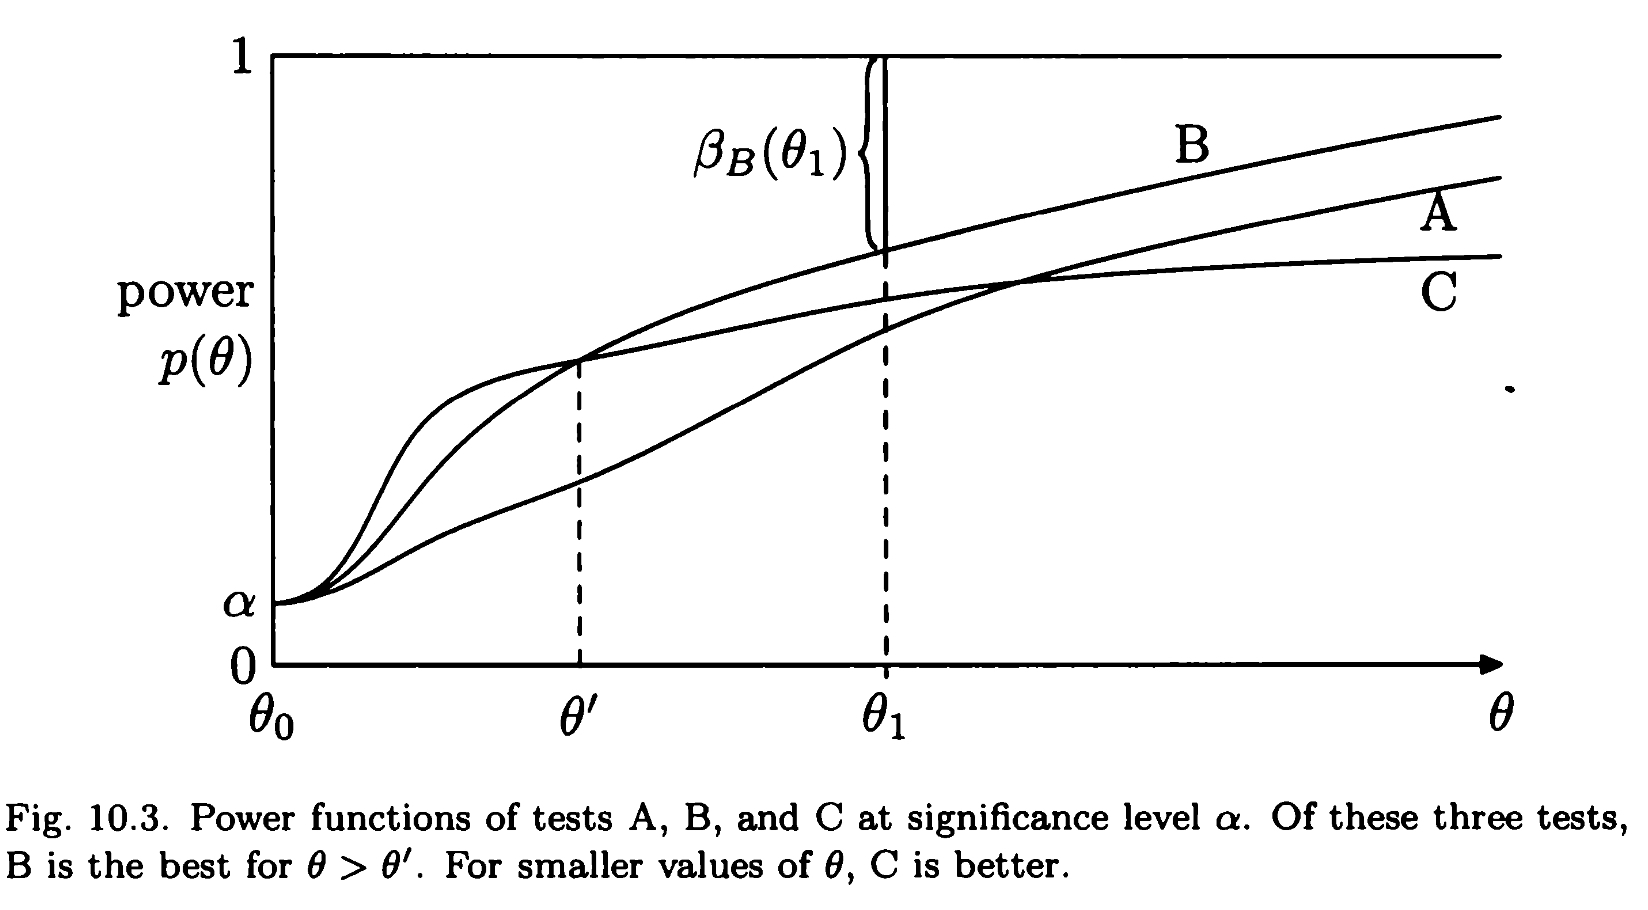
\includegraphics[trim={0cm 0cm 0 0},clip, keepaspectratio,width=0.85\textwidth]{figures/james/test/mostpower}
	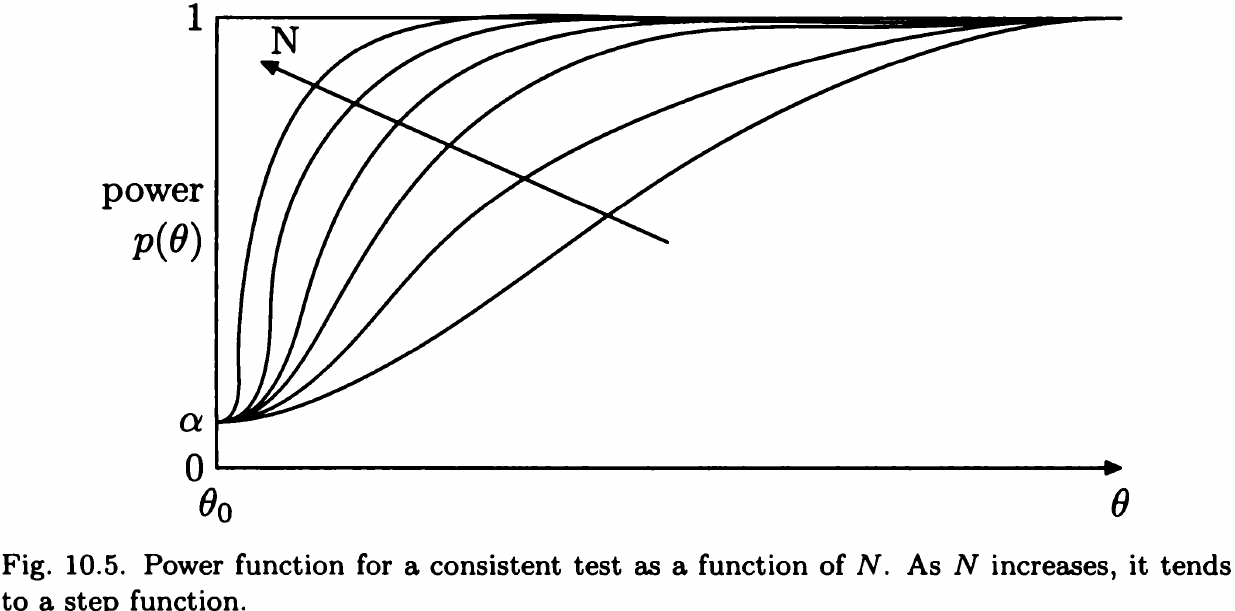
\includegraphics[trim={0cm 0 0 0},clip, width=0.85\textwidth]{figures/james/test/powerconsistent}
	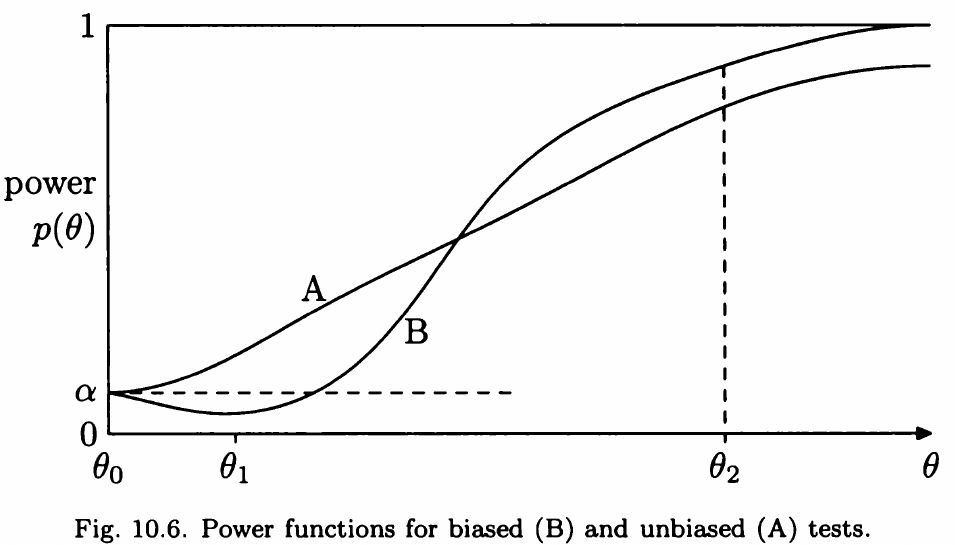
\includegraphics[trim={0cm 0 0 0},clip,width=0.8\textwidth]{figures/james/test/biasedtest}
\end{figure} 
	Test B can't distinguish between $\theta_0$, $\theta_1$.
\end{column}
\end{columns}
\end{frame}

\begin{frame}{Ipotesi semplici: Lemma di Neyman-Pearson (Test di NP)}
Posso esprimere un test in funzione di una statistica: $T(\vec{x})=T(t(\vec{x}))$ (nel caso del lemma NP la statistica \'e il LR). 
Lo spazio dei parametri \'e $\theta_0,\theta_1$. Cerco la regione $w_{\alpha}$ regione critica che massimizza power $1-\beta$ (dato $\alpha$):
\begin{align*}
&\int_{w_{\alpha}}f_N(\vec{X}|\theta_0)\,dX=\alpha\\
&\int_{w_{\alpha}}f_N(\vec{X}|\theta_1)\,dX=1-\beta\\
&=\int_{w_{\alpha}}\frac{f_N(\vec{X}|\theta_1)}{f_N(\vec{X}|\theta_0)}f_N(\vec{X}|\theta_0)\,dX=\E_{w_{\alpha}}{[\frac{f_N(\vec{X}|\theta_1)}{f_N(\vec{X}|\theta_0)}|\theta_0]}\\
&\Rightarrow l_N(\vec{X},\theta_0,\theta_1)=\frac{f_N(\vec{X}|\theta_1)}{f_N(\vec{X}|\theta_0)}\geq c_{\alpha}: H_1\ (\leq c_{\alpha}: H_0)\\
&\int_{w_{\alpha}}=\{x:I_N>c_{\alpha}\}f(x,\theta_0)\,dx=\alpha
\end{align*}
\end{frame}

\begin{wordonframe}{Regione critica: NP, il verso della disuguaglianza e il quantile}
Voglio distinguere $H_0: G(\mu_0,\sigma)$ vs $H_1: G(\mu_1>\mu_0,\sigma)$ - Lemma NP:
\begin{align*}
&\frac{L(\mu_0)}{L(\mu_1)}=\exp{\frac{1}{2\sigma}[\sum_i(x_i-\mu_1)^2-\sum_i(x_i-\mu_0)^2]}\\
&C=\{(x_i):\exp{\frac{1}{2\sigma}[\sum_i(x_i-\mu_1)^2-\sum_i(x_i-\mu_0)^2]}\leq k\}\\
&C=\{(x_i):\exv{X}\geq k'=\mu_0+\lambda_{1-\alpha}\frac{\sigma}{\sqrt{N}}\}
\end{align*}
\end{wordonframe}

\begin{frame}{Ipotesi composte}
\begin{itemize}
\item Karlin-Rubin theorem: extension of NP lemma to composite H. Scalar measurement with pdf parametrized by scalar $\theta$, if $l(x)=\frac{f(x;\theta_1)}{f(x;\theta_0)}$ is monotone non-decreasing in $x$ for any pair $\theta_1\geq\theta_0$ then test for $H_0: \theta\leq\theta_0(\theta=\theta_0)$ vs $H_1: \theta>\theta_0$ defined by threshold test function $\phi(X)=\lbt{1\ x>x_0}{0\ x<x_0}$ con $\E_{\theta_0}{[\phi]}=\alpha$
\item For exponential family exists UMP one-sided ($H_0: \theta=\theta_0$, $H_1: \theta>\theta_0$)
\item Se non esiste UMP test e ho bisogno di massima sensibilit\'a in intorno di $\theta_0$: score \'e asintoticamente normale
\[\PDy{\theta}{\ln{L}}|_{\theta_0}\gtrless\lambda_{?1-\alpha}\sqrt{NI}\]
\end{itemize}
\end{frame}

\begin{frame}{LMP test}
Se ho bisogno di massima sensibilit\'a vicino alla soglia: $1-\beta$ grande nelle vicinanze di 0: $H_0$: $\theta=\theta_0$, $H_1$: $\theta=\theta_0+\Delta$, quindi $\ln{L(\vec{X},\theta_1)}\approx\ln{L(\vec{X},\theta_0)}+\Delta\PDy{\theta}{\ln{L}}|_{\theta_0}$.
Applico NP a $H_0$ vs $H_1$:
\begin{equation*}
\ln{L(\vec{X},\theta_1)}-\ln{L(\vec{X},\theta_0)}\gtrless c_{\alpha} \Rightarrow \PDy{\theta}{\ln{L}}\gtrless q_{\alpha}
\end{equation*}
\begin{columns}[T]
	\begin{column}{0.4\textwidth}
		\begin{align*}
		&H_0: \theta=\theta_0\\
		&H_1: \theta=\theta_0+\Delta
		\end{align*}
	\end{column}
	\begin{column}{0.6\textwidth}
		\begin{align*}
		&\PDy{\theta}{\log{L}}\gtrless k_{\alpha}\gtrless\lambda_{\alpha}\sqrt{NI}\\
		&\E{[\PDy{\theta}{\log{L}}|_{\theta_0}]}=0,\ \E{[(\PDy{\theta}{\log{L}}|_{\theta_0})^2]}=NI
		\end{align*}
	\end{column}
\end{columns}
\end{frame}

\begin{frame}{LR test}
James pg 287
\end{frame}

\section{GOF}

\subsection{Binned GOF}

\begin{frame}{Pearson $\chi^2$ test for multinomial null hypothesis (histograms with k bins)}
Asymptotic normality of multinomial to find asymptotic pdf of
\[(\vec{n}-N\vec{p})^T\invers{V}(\vec{n}-N\vec{p})\]
$V$ matrice covarianza osservazioni $\vec{n}$ di rango $k-1$ visto $\sum_i^kn_i=N$. Treating all bins simmetrically we find
\[T=\frac{1}{N}\sum_i^k\frac{(n_i-Np_i)^2}{p_i}\]
distribution of T close enough to $\chi^2(k-1)$ when all expected events per bin $Np_i>5$
\end{frame}

\begin{wordonframe}{Dettagli su $\chi^2$ di pearson}
$k+1$ outcomes, n trials, $\sum_jp_j=1$, $\sum_in_i=N$: $\prob{(Y_1=y_1,\ldots,Y_{k+1}=y_{k+1})}=\frac{n!}{y_1!*\ldots*y_{k+1}!}p_1^{y_1}\ldots p_{k+1}^{y_{k+1}}$. Parameter space $\Omega=\{(p_1,\ldots,p_k\})\in \real{k}: p_i\geq0,\sum_{j=1}^kp_j\leq1$.
$H_0: p_i=\pi_i$ vs $K: p_i\neq\pi_i$:
statistica $Q_n=\sum_j^{k+1}\frac{(Y_j-n\pi_j)^2}{n\pi_j}\to\frac{1}{N}\sum^{k+1}\frac{n_i^2}{p_i}-N$ ha asintotic. pdf $\chi^2(k)$, quindi se $c_{k,1-\alpha}$ $1-\alpha$-quantile di $\chi^2(k)$ il test che rifiuta H quando $Q_n>c_{k,1-\alpha}$ ha asintoticamente valore critico $\alpha$.
\begin{block}{Power against local alternatives}
	\begin{itemize}
		\item $H: p_j=\pi_j$, $j=1,\ldots,k+1$: $Q_n\xrightarrow{d}\chi^2(k)$
		\item Under alternative hypothesis $K: p_j^{(n)}=\pi_j+n\expy{-1/2}h_j$, $\sum_jh_j=0$: $Q_n\xrightarrow{d}\chi^{2,\lambda}(k)$ and NC parameter $\lambda=\sum_j^{k+1}\frac{h_j^2}{\pi_j}$
		\item Power of $\chi^2$ test based on $Q_n$ tends to a limit greater than critical value $\alpha$
	\end{itemize}
\end{block}
\end{wordonframe}

\begin{frame}{$\chi^2$ Test of uniformity}
$X_1,\ldots,X_n$ iid RV con pdf $F$; $H: F=F_0(t)=t$ uniform cdf in $(0,1)$. Divido l'intervallo $(0,1)$ in $k+1$ sotto-intervalli di lunghezza $\frac{1}{k+1}$: pdf di $(Y_1,\ldots,Y_{k+1})$ \'e multinomiale e il test che rifiuta H per grandi $\sum_j^{k+1}\frac{(Y_j-\frac{n}{k+1})}{\frac{n}{k+1}}$.
\end{frame}

\subsection{Unbinned GOF}

\begin{frame}{Kolmogorov-Smirnov and Cramer-von Mises tests}
\begin{block}{Classes of EDF statistics}
	Empirical distribution function (EDF): N iid RV: $F_n(X)=\frac{1}{N}\sum_i^NI_{[-\infty,x](X_i)}$ $\hat{F}_n(t)=\frac{\#\text{ elementi nel campione }\leq t}{n}$.
 Ordering statistics, $X_{(1)}, X_{(2)}, \ldots X_{(N)}$, $S_N=\left\{\begin{array}{c}0\ X<X_{(1)}\\i/N\ X_{(i)}<X<X_{(i+1)}\\1\ X>X_{(N)}\end{array}\right\}$
\end{block}
%Smirnov-Cramer-von Mises test for unbinned data

\begin{block}{Test di Kolmogorov-Smirnov }
La statistica \'e massima deviazione di $S_N$ osservato da distribuzione $F(X)$ sotto $H_0$:
\begin{align*}
&D_N=\max|S_N(X)-F(X)|:\ \lim_{N\to\infty}\prob{[\sqrt{N}D_N>z]}=2\sum_{r=1}^{\infty}(-1)\expy{r-1}\exp{-2r^2z^2}\\
&D_N^{\pm}=\max\pm(S_N(X)-F(X)):\ \lim_{N\to\infty}\prob{[\sqrt{N}D_N^{\pm}>z]}=\exp{-2z^2}
\end{align*}
%$T_n=\sup_{t\in\real}{|\hat{F}_n(t)-F(t)|}$: largest of $|F_n(y_k)-F_0(y_k)|$, $|F_n(y_{k-1})-F_0(y_k)|$. Sia $s_{n,1-\alpha}$ il $1-\alpha$-quantile di $T_n$ per ogni $F$ continua: KS-test rejects H if $T_n>s_{n,1-\alpha}$.
Rejects null hypothesis at level $\alpha$ if $\sqrt{N}D_N>K_{\alpha}$ dove $K_{\alpha}$ \'e determinato tramite $\prob{[\sqrt{N}D_N<K_{\alpha}]}=1-\alpha$ (asintoticamente)
\end{block}
\end{frame}


\section{Compiti}\linkdest{compiti}

\begin{frame}[allowframebreaks]{Section TOC}
%currentsection,hideallsubsections,subsubsectionstyle=hide
\tableofcontents[currentsection,sectionstyle=show/hide,subsectionstyle=show/show/hide]
\end{frame}

\subsection{Passaggio a livello (17/09/2020)}

\begin{frame}{Tempo medio chiusura da numero di volte che \'e chiuso}
\begin{itemize}
\item Attraversamento N volte di passaggio a livello di cui k volte \'e chiuso: \keyword{k segue pdf Poisson o binom? Poisson limite grandi N, piccola probabilit\'a p e successi per unit\'a di tempo/spazio dati!}. \keyword{Quali presupposti per $p=\frac{T_c}{T_{day}}$ parametro binom con $T_c$ tempo chiuso} - ci siamo ridotti a stimare p: $\hat{p}_{MLE}=\frac{k}{N}$, $\var{\hat{p}}=\frac{Np(1-p)}{N^2}$
\end{itemize}
\end{frame}

\subsection{Dadi D\&D (28/05/18): 4,6,8,10,12,20 facce - T. prob. tot, Bayes T., stima interv.}

\begin{frame}{Probabilit\'a estrazione 1 dopo selezione dado a caso da cui \'e uscito 1}
\begin{itemize}
\item Probabilit\'a 1:
\begin{align*}
&P(1)=\sum_i^6\prob{(1|D_i)}\prob{(D_i)}=\frac{1}{6}(\frac{1}{4}+\frac{1}{6}+\frac{1}{8}+\frac{1}{10}+\frac{1}{12}+\frac{1}{20})\approx0.129\tag{T. Prob. Tot.}
\end{align*}
\item Prob. di ottenere 1 quando nella prima estrazione \'e uscito 1, $\prob{(1|1)}$:
\begin{align*}
&\prob{(1|1)}=\sum_i^6\prob{(1|D_i,1)}\prob{(D_i|1)}\tag{T. prob. Tot.}\\
&\prob{(1|1)}=\sum_i^6\frac{1}{i}\frac{\prob{(1|D_i)\prob{(D_i)}}}{\prob{(1)}}\tag{T. Bayes}
\end{align*}
Indipendenza dei due lanci: non sono indipendenti, $\prob{(1|1)}\neq\prob{(1)}$; i due eventi casuali in $\prob{(1|1)}$ il primo ''estrazione dado e lancio'', il secondo ''lancio'' - nella sommatoria entrano funzioni fattorizzabili delle variabili corr. ai risultati dei due lanci, ma la somma non \'e fattorizz.
\end{itemize}
\end{frame}

\begin{frame}{Stime intervallari su numero facce freq./Bayes.}
\begin{itemize}
\item Limiti Bayesiani al $\cred=90\%$ avendo 1 al primo lancio. Posterior ordering: $\prob{(D_i|1=\frac{1}{i\sum_j^61/j})}$ decrescente con $i$ e si hanno limiti superiori - $4\leq i\leq12$
\item Limiti frequentisti al $\cl=90\%$ sul numero di facce - \keyword{Scelta algoritmo ordinamento per costruzione banda di Neyman}: prob. ottenere n dal lancio di qualunque dado $\prob{(n|D_i)}=\frac{1}{i},\ n\leq i$ - per limiti superiori si sceglie ord. decrescente in osservabile n ($n=1\Rightarrow i\leq10$ al $\cl=90\%$)
\begin{figure}
	\centering
	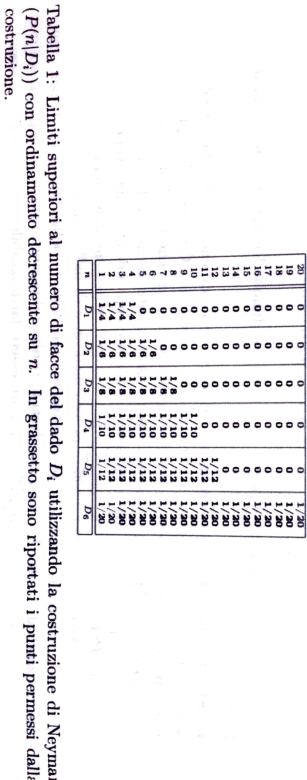
\includegraphics[angle=90,origin=c, width=0.99\textwidth,keepaspectratio]{figures/compiti/201805Neymandecreasing}
	\label{fig:201805Neymandecreasing}
\end{figure}
\end{itemize}
\end{frame}

\begin{frame}{Banda di Neyman con LR ordering a l\'a FC}
Ordinamento in base al Rapporto di Likelihood $O(D_i,n)=\lr(n)=\frac{\prob{(n;D_i)}}{\sup_{D_i'}\prob{(n;D_i')}}$: tabella 2 mostra a sinistra banda di confidenza e a destra i valori di LR.
\begin{figure}
	\centering
	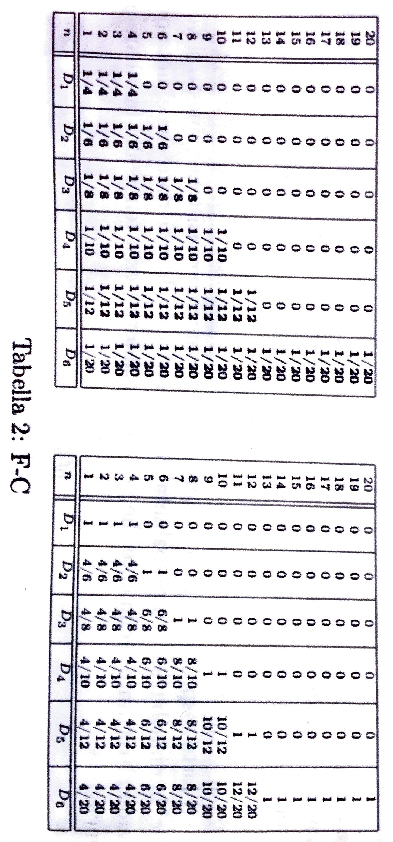
\includegraphics[angle=90,origin=c, width=0.99\textwidth,keepaspectratio]{figures/compiti/201805NeymanLR}
	\label{fig:201805NeymanLR}
\end{figure}
\end{frame}

\subsection{N numeri casuali da uniforme: stime di m da statistica minimo}

\begin{frame}{Propriet\'a statistica $x_{min}$}
	$X_{(1)}<X_{(2)}<\ldots<X_{(n)}$: pdf $\prob{(X_{(k)}\in[x,x+dx])}$
\begin{block}{Maximum/minimum statistics}
	\begin{align*}
	&\prob{(X_{(1)}<x)}=1-\prob{(X_{(1)}>x)}\\
	&=1-\prob{(X_1>x)}\ldots\prob{(X_n>x)}=1-[1-F(x)]^n\\
	&\prob{(X_{(n)}<x)}=\prob{(X_1<x,\ldots,X_n<x)}=F(x)^n
	\end{align*}
\end{block}
Pdf di $x_m$ derivando cumulante o usando simmetria pdf uniforme sotto trasformazione $x\to m-x$: $\prob{(x_m)}=\frac{N}{m}(1-\frac{x_m}{m})^{N-1}$:
\begin{align*}
&\E{[x_m]}=\int\delta_{[0,m]}x_m\frac{N}{m}(1-\frac{x_m}{m})^{N-1}\,dx_m=\frac{N}{m}[-\frac{m}{N}(1-\frac{x_m}{m})^{N-1}x_m|_0^m+\int\frac{m}{N}(1-\frac{x_m}{m})^N\,dx_m]\\
&=\frac{N}{m}\frac{m}{N}[-\frac{m}{N+1}(1-\frac{x_m}{m})^{N+1}]|_0^m=\frac{m}{N+1}\\
&\var{[x]}=\E{[(x-\mu)^2]}=\E{[x^2]}-\mu^2=\int_0^mx_m^2\frac{N}{m}(1-\frac{x_m}{m})^{N-1}\,dx_m-(\frac{m}{N+1})^2=\frac{N}{(N+1)^2(N+2)}m^2
&\E{[X^2]}-(\E{[X]})^2\geq0\tag{Jensen ineq.}
\end{align*}
\keyword{$x_m$ non \'e stat. suff per $U([0,m])$}: mentre fissando $x_m$ le altre osservazioni sono indipendenti da m, per il minimo l'estremo superiore rimane ignoto.
\end{frame}

\begin{frame}{Stimatore estremo superiore U da minimo campionario}
\begin{columns}[T]
\begin{column}{0.5\textwidth}
\begin{align*}
&\hat{m}=Nx_m\\
&\E{[\hat{m}]}\to m\tag{asynt.unbias.}\\
&\hat{m}'=\frac{N+1}{N}\hat{m}=(N+1)x_m\tag{unbias.}\\
&\var{\hat{m}'}=\frac{N}{N+2}m^2
\end{align*}
\end{column}
\begin{column}{0.5\textwidth}
$\hat{m}'$ non \'e consistente: $\lim_{n\to\infty}T_n(X_i)\xrightarrow{P}\tau(\theta)$
\begin{align*}
&\prob{\hat{m};m}=\frac{N}{m}(1-\frac{\hat{m}}{(N)m})^{N-1}\frac{d\hat{m}}{N}\to\frac{1}{m}\exp{-\frac{\hat{m}}{m}}
\end{align*}
''non diventa piccata attorno al valore vero m per N grandi'': lo stimatore \'e inconsistente
\end{column}
\end{columns}
\end{frame}

\begin{frame}{limit di confidenza frequentisti da $x_m$}
\begin{columns}[T]
	\begin{column}{0.5\textwidth}
		Limiti superiori: ordinamento $x_m\geq x_1$
		\begin{align*}
		&\int_{x_1}^{m}\frac{N}{m}(1-\frac{x_m}{m})^{N-1}\,dx_m=\cl\\
		&m\leq\frac{x_m}{1-\cl^{\frac{1}{N}}}
		\end{align*}
	\end{column}
	\begin{column}{0.5\textwidth}
\def\myscale{0.4}
\begin{tikzpicture}[myscale]
\begin{axis}[title={Banda confidenza: $o:x_m\geq x_1$},name=uniformconfidence,ymin=0,xmin=0,xmax=8,xlabel={$m$},ylabel={$x$},y label style={rotate=-90, at={(-0.1,1.)}},extra x tick style={% changes for extra x ticks
	tick label style={yshift=0mm}},extra y ticks={0.3},extra y tick labels={measure $x_0$}]
\addplot[name path global=bp, no marks] gnuplot[id=upperbound,domain=0:8] {x*(1-0.9)};
%\addplot[name path global=bm, no marks] gnuplot[id=lowerbound,domain=0:8] {x};
%\addplot[name path global=meas,dash pattern=on 4pt off 3pt,no marks,black] gnuplot[domain=0:8] {0.3};
%\path[name intersections={of={bp and meas},name=i},name intersections={of={bm and meas},name=j}] (i-1) (j-1);
%\pgfplotsextra{\path (i-1) \pgfextra{\markxof{i-1}\xdef\myfirsttick{\pgfmathresult}}(j-1); \pgfextra{\markxof{j-1}\xdef\mysecondtick{\pgfmathresult}};
%}
\end{axis}
%\draw[ultra thin, draw=gray] (i-1 |- {rel axis cs:0,0}) node[fill=yellow,yshift=-1ex]{\pgfmathprintnumber[fixed,precision=5]\myfirsttick} -- (i-1);
%\draw[ultra thin, draw=gray] (j-1 |- {rel axis cs:0,0}) node[fill=red,below]{\pgfmathprintnumber[fixed,precision=5]\mysecondtick} -- (j-1);
\end{tikzpicture}
	\end{column}
\end{columns}
\end{frame}

\subsection{2 numeri casuali da pdf uniformi (21/11/19)}

\begin{frame}{Joint pdf, marginalization (and \keyword{integration limits})}
	Scelti 2 numeri casuali da $U(0,m)$, con ipotesi provenienza da $U(0,x_1)$ ($x_+=\max{[x_1,x_2]}$, $x_-=\min{[x_1,x_2]}$) - joint pdf $	P(x_-,x_+)=\frac{1}{m^2}$ per lálgoritmo giusto, 
	\begin{align*}
	&\prob{(x_-)}=\int\prob{(x_-,x_+)}\,dx_+=\int\frac{I(0\leq x_-\leq x_+\leq m)}{(m?)x_+}\,dx_+\\
	&=\int_{x_-}^m\frac{dx_+}{x_+m}=\frac{1}{m}\ln{\frac{m}{x_-}}\\
	&\prob{(X_-<x_1|X_+=x_+)}\lbt{1:\ x_+<x_-}{\frac{x_-}{x_+}:\ x_-<x_+}\\
	&\prob{(X_-<x_-)}=\int_{x_+=0}^{x_-}\,dx_++\int_{x_+=x_-}^1\frac{x_-}{x_+}\,dx_+\\
	&P(x_+)=\frac{1}{m},\ P(x_-)=\frac{1}{m}\ln{\frac{m}{x_-}}
	\end{align*}
\end{frame}

\begin{frame}{Test ipotesi (significato) e moment estimator}
	Test per identificare algoritmo sbagliato da parte di studente: \keyword{RV come parametro $U$ e ipotesi semplici} (nel caso del singolo studente ho tutti i parametri fissi) - significato del test (cosa significa che su 20 trovo 6 casi?) - cosa combia sapendo che su un grande campione risulta che $5\%$ studenti usano algoritmo sgabliato? Quale probabilit\'a che studente positivo abbia usato algoritmo sbagliato?
	Stimare col metodo dei momenti la frazione di studenti che usa algoritmo sbagliato avendo a disposizione lista di tutti numeri generati: $\int(x-\frac{m}{2})[(1-f)\frac{1}{m}+\frac{f}{m}\ln{\frac{m}{x}}]\,dx\approx\frac{2f}{N}\E{[x_-]}$??.
		Local most powerfull test having $x_-$ to determine even small fraction of wrong algoritm: test statistics??
		\begin{align*}
		&\TDof{f}\ln{L(\vec{X},f)}|_{\theta=0}
		\end{align*}
	\end{frame}

\begin{frame}{Test, ipotesi semplice e pdf uniforme}
Lista completa $(x_+,x_-)$. Test per distingure: tutti algoritmo giusto da tutti algoritmo sbagliato.
Considero $H_0$: $x_-\in U(0,m)$, $H_1$: $x_-\in U(0,x_+)$. Statistica di test e distribuzione sotto le due ipotesi?
\begin{align*}
&T(\vec{X})=\prod_i^N\frac{m}{x_{+i}}I(0\leq x_{-i}\leq x_{+i})\tag{NP}
\end{align*}
Pdf asintotica statistica, soglia regione critica e power per $\alpha=0.1$.

\end{frame}

\subsection{{Combinazione p-value per 10 osservabili indipendenti (16/07/18)}}
\begin{frame}{Valori $\chi^2$ per 10 osservabili binned}
	Fit di massima likelihood per le 10 osservabili (binned) basandosi su teoria: istogrammi suff. popolati per GOF test di Pearson con 30 dof (31 bins?)
	\begin{table}[h!]
		\centering
		\begin{tabular}{||cccccc||} 
			$\chi^2(/30?)$&38.33&40.87&30.70&36.91&39.97\\
			&36.97&20.48&32.34&41.32&41.41\\
			$P(\chi^2_{30}<x)$&0.859&0.911&0.570&0.820&0.894\\
			&0.822&0.096&0.648&0.918&0.920\\
		\end{tabular}
	\end{table}
	Impressione che ci siano troppi valori alti del $\chi^2$: come risolvere il dubbio in maniera rigorosa?
\end{frame}
\begin{frame}{Additivit\'a $\chi^2$ e GOF test}
	\begin{itemize}
	\item \keyword{additivit\'a del $\chi^2$}: somma quadrati di RV normali standard.
			Sommando $\chi^2$ in tab si ottiene RV con pdf $\chi^2_{300}$ approssimabile con gaussiana con $\sigma=\sqrt{2N}\approx24.5$.
			$\sum_i\chi^2_i=359.3$, siamo a $1.21\sigma$
	\item KS test: campione di 10 valori in accordo con pdf $\chi^2_{30}$ (cumulante $\prob{(\chi^2_{30}<x)}$ in tabella). Calcolo $F_n(x_{k-1})-F_n(x_k)$ e $F_n(x_k)-F_n(x_k)$:  $|0-0.096|$, $|0.1-0.57|$, $|0.2-0.648|$, $|0.3-0.82|$, $|0.4-0.822|$, $|0.5-0.859|$, $|0.6-0.894|$, $|0.7-0.914|$, $|0.8-0.918|$, $|0.9-0.926|$; $\Delta=0.52$??
	\item Combinazione diretta p-values: $p_i=1-\prob{(\chi^2_{30}<x)}$, pdf somma log p-values $-2\log{(\prod^Np_i)}$ ha pdf $\chi^2_{2N}$
	\item Test binned: hist of p-values (3-4) e considero LR con pdf uniforme (pdf p-value) e quindi usarlo per test basato su pdf asintotica (esatta, calcolandola)
	\item Considerare max(min) dei p-values e usare pdf $x_M$ per test
	\item Test della mediana
	\item Test basato su propriet\'a pdf $\chi^2_{30}$: test varianza $2N$; test secondo momento attorno a media nominale 30.
\end{itemize}
\end{frame}

\begin{frame}{Stimatori, confidence/credible interval per parametro m di pdf uniforme da misura della mediana(16/07/18)}
\begin{columns}[T]\begin{column}{0.5\textwidth}
x RV $U(0,m)$; $2k+1=3$ misura la mediana $x_2=3.4$
\begin{block}{MLE estimator, bias, incertezza statistica}
\begin{align*}
&\prob{(\mu=x_2)}=6\frac{\mu}{m^2}(1-\frac{\mu}{m})\\
&\hat{\mu}_{MLE}=3/2\mu\\
&\E{[\hat{m}]}=\frac{3}{2}\E{[\mu]}\frac{3}{2}\int_0^{m}\mu\prob{(\mu)}\,d\mu\\
&=\frac{3}{4}m\\
&\hat{m}'=\frac{4}{3}\hat{m}=2\mu\\
&\var{[\hat{m}]}=\sigma^2_{\hat{m}}=\frac{9}{4}\var{\mu}=\frac{9}{4}\sigma_{\mu}^2\\
&\var{[\hat{m}']}=\sigma^2_{\hat{m}'}=4\var{\mu}=4\sigma_{\mu}^2\\
&\sigma^2_{\mu}=\exv{\mu^2}-\exv{\mu}^2=\frac{m^2}{20}
\end{align*}
Le varianze sono funzione del valore di m: le stimo usando $\hat{m}$
\end{block}
\end{column}\begin{column}{0.5\textwidth}
Likelihood pdf uniforme: \begin{equation*}L_x(m)=\left\{\begin{array}{c}
0\ m<x\\
1/m\ m\geq x\\
\end{array}\right.
\end{equation*}
Determinazione $p(\mu=x_2)$ dove $\mu$ pu\'o essere vista come seconda misura pi\'u grande o mediana; per $2k+1$ misure
\begin{align*}
&\prob{(\mu;m)}=\prob{(\mu)}F(\mu)^k[1-F(\mu)]^k\\
&(2k+1)\binom{2k}{k}\\
&\prob{(\mu;m)}=\frac{1}{m}(\frac{\mu}{m})^k(1-\frac{\mu}{m})^k\frac{(2k+1)!}{k!k!1!}
\end{align*}
\vspace{5cm}
\begin{block}{Stima bayesiana di m}
Assumo prior uniforme in $\log{m}$: $\prob{(m)}\propto\frac{1}{m}$, posterior $\pi(m)\propto L(\mu|m)\prob{(m)}=\frac{6\mu}{m^3}-\frac{6\mu^2}{m^4}$ ($\prob{(H)}=\frac{\prob{(E|H)\prob{(H)}}}{\prob{(E)}}$): la posterior va normalizzata tra $[\mu,+\infty]$ (likelihood nulla  in $[0,\mu]$), $\pi(m)=\frac{3\mu^2}{m^3}-\frac{3\mu^3}{m^4}$, il massimo fornisci una stima bayesiana di m: $\hat{m}=\frac{4}{3}\mu$.
\end{block}
\end{column}\end{columns}
\end{frame}

\begin{frame}{Stimatori, confidence/credible interval per parametro m di pdf uniforme da misura della mediana(16/07/18)}
\begin{columns}[T]\begin{column}{0.5\textwidth}
\begin{block}{MLE estimator, bias, incertezza statistica}
\begin{align*}
&\var{[\hat{m}']}=\sigma^2_{\hat{m}'}=4\var{\mu}=4\sigma_{\mu}^2\\
&\sigma^2_{\mu}=\exv{\mu^2}-\exv{\mu}^2=\frac{m^2}{20}
\end{align*}
Le varianze sono funzione del valore di m: le stimo usando $\hat{m}$
\end{block}
\end{column}\begin{column}{0.5\textwidth}
\begin{block}{Stima bayesiana di m}
Assumo prior uniforme in $\log{m}$: $\prob{(m)}\propto\frac{1}{m}$, posterior $\pi(m)\propto L(\mu|m)\prob{(m)}=\frac{6\mu}{m^3}-\frac{6\mu^2}{m^4}$ ($\prob{(H)}=\frac{\prob{(E|H)\prob{(H)}}}{\prob{(E)}}$): la posterior va normalizzata tra $[\mu,+\infty]$ (likelihood nulla  in $[0,\mu]$), $\pi(m)=\frac{3\mu^2}{m^3}-\frac{3\mu^3}{m^4}$, il massimo fornisci una stima bayesiana di m: $\hat{m}=\frac{4}{3}\mu$.
\end{block}
\end{column}\end{columns}
\end{frame}

\begin{frame}{Limite di confidenza superiore/bilaterale}
Limite superiore per m di $U(0,m)$ da mediana campionaria: $\int_{\mu}^m6\frac{\tilde{\mu}}{m^2}(1-\frac{\tilde{\mu}}{m})\,d\tilde{\mu}=\cl=0.9$, con $y=\frac{\mu}{m}$ si risolve $F(\mu)=y^2(3-2y)=1-\cl$ ha soluzione $y=0.1958$ quindi $m<\frac{\mu}{0.1958}$.
Limite bilaterali simmetrici per m da mediana campionaria: $F(\mu)=y^2(3-2y)=(1-\cl)/2$ $y_+=0.13535$, $\int_{\mu}^m6\frac{\tilde{\mu}}{m^2}(1-\frac{\tilde{\mu}}{m})\,d\tilde{\mu}=(1-\cl)/2$ quindi $F(\mu)=y^2(3-2y)=(1+\cl)/2$ e $y_-=0.8647$: Limiti bilaterali con $\cl=0.9$ sono $\frac{\mu}{0.8647}<m<\frac{\mu}{0.13535}$
\end{frame}

\begin{frame}{Limiti credibilit\'a Bayesiana}
prior uniform, $\cred=90\%$. La posterior \'e $\pi(m)=\frac{2\mu}{m^2}-\frac{2\mu^2}{m^3}$ diversa da zero in $[\mu,+\infty]$ e la cumulante $F(m)=\int_{\mu}^m\pi(\tilde{m})\,d\tilde{m}=1+\mu(\frac{\mu}{m^2}-\frac{2}{m})$:
\begin{align*}
&F(m_{min})=\frac{1-\cl}{2}\\
&F(m_{max})=\frac{1+\cl}{2}\\
&\frac{\mu}{1-\sqrt{(1-\cl)/2}}<m<\frac{\mu}{1-\sqrt{(1+\cl)/2}}
\end{align*}
dove ho scelto le soluzioni maggiori di $\mu$, per il limite superiore si ha $m<66.26$.
\end{frame}

\begin{frame}{Limiti confidenza al $90\%\cl$ \'a l\'a FC}
Imponiamo il LR-ordering e coverage $90\%$
\begin{equation*}
\lambda\propto\mu\prob{(\mu;m)}=6\frac{\mu^2}{m^2}(1-\frac{\mu}{m})
\end{equation*}
LR \'e unimodale: un intervallo con $\lambda(m_1)=\lambda(m_2)$, mentre il coverage richiede $\int_{m_1}^{m_2}\prob{(\mu;m)}\,d\mu=\cl$ da cui si ottiene il sistema di equazioni
\begin{align*}
&y_2^3-y_1^3=\cl\\
&y_2^2-y_1^2=\cl\\
&y_1=\frac{m_1}{m},\ y_1=\frac{m_1}{m}\\
&\frac{\mu}{0.96804}<m<\frac{\mu}{0.192606}
\end{align*}
\end{frame}

\begin{frame}{$2k+1$ misure: propriet\'a statistica mediana per costruzione estimatori}
pdf per mediana campionaria
\begin{equation*}	\prob{(\mu;m)}=\frac{1}{m}(\frac{\mu}{m})^k(1-\frac{\mu}{m})^k\frac{(2k+1)!}{k!k!1!}
\end{equation*}
stimatore massima likelihood:
\begin{align*}
&\log{L(m)}=\log{\frac{1}{m}}+k\log{\frac{\tilde{m}}{m}}+k\log{(1-\frac{\tilde{m}}{m})}+\const{}\\
&\TDy{m}{\log{L}}=0 \Rightarrow \hat{m}=\frac{2k+1}{k+1}\tilde{m}
\end{align*}
Bias estimatore:
\begin{align*}
&\E{[\hat{m}]}=\frac{2k+1}{k+1}\E{[\tilde{m}]}\\
&\E{[\tilde{m}]}=\int_0^m\tilde{m}\prob{(\tilde{m};m)}\,d\tilde{m}\\
&=\frac{(2k+1)!}{k!k!1!}m\int_0^1x^{k+1}(1-x)^k\,dx\ (x=\frac{\tilde{m}}{m})\\
&\E{[\tilde{m}]}=\frac{(2k+1)!}{k!k!1!}m\frac{\Gamma(k+1)\Gamma(k+2)}{\Gamma(2k+3)}=\frac{m}{2}\ (\Gamma(k+1)=k!)\\
&\E{[\hat{m}]}=\frac{2k+1}{2(k+1)}m\\
&b=m-\frac{2k+1}{2(k+1)}=\frac{1}{2(k+1)}m\to0
\end{align*}
Varianza
\begin{align*}
&\E{[\tilde{m}^2]}=\frac{(2k+1)!}{k!k!1!}m^2\int_0^1x^{k+2}(1-x)^k\,dx\\
&=\frac{(2k+1)!}{k!k!1!}m^2\frac{\Gamma(k+1)\Gamma(k+3)}{\Gamma(2k+4)}\\
&=\frac{(k+1)(k+1)}{(2k+3)(2k+2)}m^2\\
&\var{[\tilde{m}]}=\E{[\tilde{m}^2]}-\E{[\tilde{m}]}^2=m^2\frac{1}{4(2k+3)}\\
&\var{[\hat{m}]}=(\frac{2k+1}{k+1})^2\var{[\tilde{m}]}\to0
\end{align*}
Efficienza estimatore mediana campionaria per pdf uniforme: non si pu\'o usare MVB come riferimento assoluto dato che per pdf uniforme $I_F$ non \'e proporzionale al numero di misure; efficienza relativa rispetto a stimatore ricavato da statistica suff. $x_M$ $\var{[x_M]}=frac{m^2}{k^2}$: il MLE ricavato da mediana \'e meno efficiente ed efficienza relativa va a 0.
\end{frame}

\subsection{Stime limite superiore dati da pdf uniforme (Problema 1 - Compito $09/11/18$)}

\begin{frame}{Pdf secondo valore pi\'u grande $x_2$}
pdf di $X_{(2)}$ per N estrazioni da pdf uniforme:
\begin{align*}
&\prob{(X_{(k)}<x)}=\sum_{i=k}^nc(n,i)F(x)^i[1-F(x)]^{n-i}\\
&\PDof{p}\sum_{i=k}^nc(n,i)p^{i}[1-p]^{n-i}=nC(n-1,k-1)p\expy{k-1}(1-p)\expy{k-1}\\
&\prob{(X_{(k)})}=nC(n-1,k-1)f(x)F(x)\expy{k-1}(1-F(x))\expy{k-1}\\
&\prob{(x_2;m)}=N(N-1)\frac{1}{m^N}x_2\expy{N-2}(m-x_2)
\end{align*}
\end{frame}

\begin{frame}{Confronto efficienza stimatore da $x_2$ vs $x_M$}
\begin{columns}[T]
\begin{column}{0.5\textwidth}
Efficienza stimatore di m da statistica $x_2$:\\
Massimizzando $L(m)$ per m si ha $\hat{m}=\frac{N}{N-1}x_2$\\
bias $\E{[\hat{m}]}-m=-\frac{1}{N+1}m$:\\ $\hat{m}'=\frac{N+1}{N}\hat{m}=\frac{N+1}{N-1}x_2$\\
varianza $\var{[\hat{m}']}=\E{[\hat{m}'^2]}-\E{[\hat{m}']}^2$
\begin{align*}
&\E{[\hat{m}'^2]}=\frac{(N+1)^2}{(N-1)^2}\E{[x_2^2]}\\
&=\frac{2}{(N-1)(N+2)}m^2
\end{align*}
\end{column}
\begin{column}{0.5\textwidth}
Efficienza $x_M$:\\
$\hat{m}_{MLE}=x_M$, stimatore unbiased $\hat{m}'=\frac{N+1}{N}\hat{m}$:
\begin{align*}
&\prob{(x_M)}=\frac{N}{m}(\frac{x_M}{m})^{N-1}\\
&L_{x_M}(m)=I_{x>M}\frac{1}{m}
\end{align*}
varianza di $\hat{m}'$:
\begin{align*}
&\E{[\hat{m}'^2]}-\E{[\hat{m'}]}^2=\frac{(N+1)^2}{N^2}\frac{N}{N+2}m^2-m^2\\
&=\frac{1}{N(N+2)}m^2
\end{align*}
efficienza relativa
\begin{equation*}
\epsilon_r=\frac{\var{[\hat{m'}_{M}]}}{\var{[\hat{m'}_{x_2}]}}
\end{equation*}
\end{column}
\end{columns}
\end{frame}

\begin{frame}{Ripetizione misure $x_2$}
Combinazione likelihood 2 misure di $x_2$: MLE massimizzando likelihood combinata
\begin{align*}
&L(m_1,m_2;x_2'x_2'')=N^2(N-1)^2\frac{1}{m^{2N}}{x_2'}^{N-1}{x_2''}^{N-2}(m-x_2')(m-x_2'')\\
&2(N-1)m^2+(x_2'+x_2'')(2N-1)m-2N(x_2'x_2'')=0\\
&\hat{m}_{\pm}=\frac{(x_2'+x_2'')(2N-1)\pm\sqrt{(x_2'+x_2'')^2(2N-1)^2-16N(N-1)x_2'x_2''}}{4(N-1)}
\end{align*}
Asintoticamente $\hat{m}=\max{(x_2',x_2'')}$ (Assumo $x_2''>x_2'$)
\end{frame}

\begin{frame}{Monotone LR}
Test bilaterale di ipotesi composte: dati da pdf uniforme con $m_1\neq m_2$? \\
Likelihood ratio test:
\begin{equation*}
\lambda(x_1',x_2'')=-2\log{\frac{\sup_m{p(x_2',x_2'';m)}}{\sup_{m_1,m_2}{p(x_2',x_2'';m_1,m_2)}}}
\end{equation*}

\begin{align*}
&\hat{m}=f(N)x_2\Rightarrow p(x_2',\hat{m})=G(N)/x_2',\ p(x_2'',\hat{m})=G(N)/x_2''\\
&\sup_{m_1,m_2}{p(x_2',x_2'';m_1,m_2)}\propto\frac{1}{x_2'x_2''},\ p(x_2',x_2'';m)\propto(m-x_2')(m-x_2'')(x_2'x_2'')^{N-2}\\
&??\sup_{m}p(x_2',x_2'';m)\propto x_2''(x_2''-x_2')(x_2'x_2'')^{N-2}
\end{align*}
Likelihood ratio monotona (asintoticamente): statistica $t(x_2',x_2'')=x_2''/x_2'$: il test LR \'e della forma $x_2''/x_2'>q_{\alpha}$
Monotone LR in statistic $T(x)$ and Karlin-Rubin theorem
\end{frame}

\subsection{Stima di tempo medio tra eventi di onde gravitazionali - problema 2 Compito $09/11/18$}

\begin{frame}{Pdf tempo tra eventi Poissoniani: MLE per eventi che generano onde gravitazionali - propriet\'a dello stimatore per numero eventi annuali}

Conteggi generati da eventi casuali statisticamente indipendenti: distribuzione del tempo tra due eventi (Poissoniana con $n\approx1$) esponenziale $\prob{(t;\tau)}=\frac{1}{\tau}\exp{-\frac{t}{\tau}}$. Il massimo della likelihood ci fornisce stimatore $\hat{t}=t_m=\SI{39}{\day}$ quindi ha la stessa distribuzione esponenziale dei tempi t: $\E{[\hat{\tau}]}=\tau$, $\var{[\tau]}=\tau^2$ quindi $\hat{\tau}=\SI{0.107+-107}{\year}$.
Il MLE trasforma in modo banale sotto cambio di variabile: $\hat{\lambda}=\hat{\frac{1}{\tau}}=\SI{9.3}{\counts\per\year}$; usando formula per propagazione errori si ha
\begin{equation*}
\sigma(\lambda)=\sqrt{\var{[\hat{\lambda}]}}\approx\frac{1}{\tau^2}\sqrt{\var{[\tau]}}
\end{equation*}
Tuttavia l'approssimazione quasi lineare del cambio di variabile \'e una pessima approssimazione sull'ampio intervallo di incertezze della variabile originale.
La distribuzione di $\hat{\lambda}=\frac{1}{\hat{\tau}}$ \'e:
\begin{equation*}
\prob{(\hat{\lambda},\lambda)}=\prob{(\hat{\tau}(\hat{\lambda});\lambda=\frac{1}{\tau})}|\TDy{\hat{\lambda}}{\hat{\tau}(=\frac{1}{\hat{\lambda}})}|
\end{equation*}
Momenti di ordine $>0$ non esistono: $\var{[\lambda]}=\infty$.
\end{frame}

\begin{frame}{Limiti di confidenza su numero eventi annuali: p-ordering, limite inferiore, LR-ratio di $\lambda$}

Stima intervallare di $\lambda=\frac{1}{\tau}$ e $\prob{(t;\lambda)}=\lambda\exp{-\lambda t}$: pdf \'e monotona decrescente in t quindi p-ordering equivale a $o(t)=-t$, $t\leq t_{max}(\lambda)$
\begin{align*}
&\int_0^{t_{max}}\lambda\exp{-\lambda t}\,dt=\cl{}:\ t_{max}(\lambda)=-\frac{\log{(1-\cl{})}}{\lambda}
\end{align*}
$t_{max}(\lambda)$ decrescente in $\lambda$, da $t<t_{max}(\lambda)$ si vede che la banda di confidenza \'e della forma $t<t_{max}(\lambda)$ porta a limite $\lambda\leq\lambda_{max}$ (limite superiore); l'inversione porta a $\lambda_{max}=-\frac{\log{(1-\cl{})}}{t_m}$.
Ma limite inferiore a un fenomeno nuovo! $o(t)=t$:
\begin{equation*}
\int_{t_{min}}^{\infty}\lambda\exp{-\lambda t}\,dt=\cl{}\Rightarrow t_{min}(\lambda)=-\frac{\log{(\cl{})}}{\lambda}
\end{equation*}
banda della forma $t\geq t_{min}(\lambda)$ porta, essendo $t_{min}(\lambda)$ decrescente il $\lambda$, a limite inferiore $\lambda\geq\lambda_{min}=-\frac{\log{(\cl{})}}{t_m}$. 

LR-ordering:
\begin{equation*}
\lr{}=\frac{\prob{(t;\lambda)}}{\sup_{\lambda}\prob{(t;\lambda)}}=\lambda t\exp{-\lambda t}
\end{equation*}
fissato $\lambda$ ha singolo massimo in t e monotona da ambo i lati: usando $o(t)=\lr{(t)}$ ottengo intervallo $[t_{min},t_{max}]$.
\end{frame}

\begin{frame}{Limiti di credibilit\'a (Bayesiani)}
Prior impropria: in mancanza di una scala definita utilizzo prior uniforme in $[0,\infty]$ (non normalizabile). Devo normalizare la posterior:
\begin{align*}
&\pi(\lambda|t_m)\propto \lambda\exp{-t_m\lambda}=L_{t_m}(\lambda)\\
&\pi(\lambda|t_m)=t_m^2\lambda\exp{-t_m\lambda}
\end{align*}
\begin{columns}[T]
	\begin{column}{0.5\textwidth}
Limite bayesiano inferiore
\begin{equation*}
\int_{\lambda_{min}}^{\infty}t_m^2\lambda\exp{-t_m\lambda}\,d\lambda=\cl{}
\end{equation*}
	\end{column}
	\begin{column}{0.5\textwidth}
Limite bayesiano bilaterale simmetrico:
\begin{align*}
&\int_0^{\lambda_{min}}t_m^2\lambda\exp{-t_m\lambda}\,d\lambda=\frac{1-\cl}{2}\\
&\int_{\lambda_{max}}^{\infty}t_m^2\lambda\exp{-t_m\lambda}\,d\lambda=\frac{1-\cl}{2}
\end{align*}
\end{column}
\end{columns}
Limite bayesiano utilizzando posterior ordering:
\begin{align*}
&\exp{-t_m\lambda_{min}}(t_m\lambda_{min}+1)-\exp{-t_m\lambda_{max}}(t_m\lambda_{max}+1)=\cl\\
&\lambda_{min}\exp{-t_m\lambda_{min}}-\lambda_{max}\exp{-t_m\lambda_{max}}=0
\end{align*}
\end{frame}

\subsection{Modello goal fatti durante partita come realizzazione poissoniana - Compito del $10/09/18$}

\begin{frame}{Modello di partita di calcio - approccio Bayesiano per determinare probabilit\'a della forzo di una squadra e del risultato successivo}
Probabilit\'a che squadra A faccia gol in un minuto \'e $q_A$: la probabilit\'a che un'incontro A-B finisca $g_A-g_B$ \'e
\[P(g_ag_B=\exp{-\mu_A-\mu_B})\frac{\mu_A\expy{g_A}\mu_B\expy{g_B}}{g_A!g_B!}\] con $\mu_i=90*q_i$.
Sia un risultato $(0,1)$: utilizzo approccio bayesiano per determinare la probabilit\'a della ''forza'' della squadra
\[\pi(g_A,g_B)=L_{0-1}(g_A,g_B)p(g_A)p(g_B)\propto\mu_2\exp{-(\mu_1+\mu_2)}\]
La probabilit\'a $P(q_A>q_B)$ integro la posterior su $dq_Adq_B$ sopra la retta $q_A=q_B$. Per determinare la probabilit\'a che in successivo incontro si abbia uno $0-0$ o $1-0$ uso la posterior calcolata in seguito allo $0-1$ che pesa le poissoniane integrati sui valori dei parametri:
\[P(g_A,g_B)=\int P(g_A,g_B;\mu_1,\mu_2)\pi(\mu_1,\mu_2)\,d\mu_1\,d\mu_2\]
\end{frame}

\begin{frame}{Test verifica modello con LRT e $\chi^2$-Pearson}
La verifica del modello tramite il confronto con risultati di 3 partite per squadra con 8 squadre: quindi confronto l'ipotesi che i gol fatti nelle tre partite da una squadra appartengano a singola Poissoniana con un modello in cui ogni risultato viene da Poisson diversa:
\[\lambda=-2\log{LR}=2\sum g_{ij}\log{\frac{g_{ij}}{\exv{g_i}}}\]
$\prob{(\lambda)}\to\chi^2_{16}$ (24-8=8*(3-1)); usando il test di Pearson $\chi^2=\sum_{ij}\frac{g_{ij}-\exv{g_i}}{\exv{g_i}}$
\end{frame}

\subsection{Contaminazione radioattiva - Compito del $10/09/18$}

\begin{frame}{Determino livello contaminazione $\alpha$ da conteggi nel tempo}
$^{32}P$, $t_{1/2}^{32}=\SI{14.263}{\day}$ di cui voglio misurare livello contaminazione $\alpha$ con isotopo raro $^{33}P$, $t_{1/2}^{33}=\SI{25.25}{\day}$. Misuro conteggi particelle beta con rivelatore a stessa ora del giorno per 5 giorni $\{n_1,\ldots,n_5\}$.\\
Ignorando fattori dipendenti solo dai dati
\begin{align*}
&\log{L(N_0,\alpha)}=\sum_{i=1}^5(n_i\log{\mu_i(N_0,\alpha)}-\mu_i(N_0,\alpha))\\
&\mu_i(N_0,\alpha)=N_0[(1-\alpha)\lambda\exp{-\lambda t_i}+\alpha\lambda'\exp{-\lambda't_i}]
\end{align*}
\end{frame}

\begin{frame}{Likelihood equation e stima con 2 conteggi}
Le likelihood equations per determinare stimatore $\hat{\alpha}$:
\begin{align*}
&\PDy{N_0}{\log{L(N_0,\alpha)}}=\sum_{i=1}^5(\PDy{N_0}{\mu_i}[\frac{n_i-\mu_i}{\mu_i}])=0\\
&\PDy{\alpha}{\log{L(N_o,\alpha)}}=\sum_{i=1}^5(\PDy{N_0}{\mu_i}[\frac{n_i-\mu_i}{\mu_i}])=0
\end{align*}
i conteggi hanno pdf Poisson centrata attorno al valore atteso determinato da numero atomi radioattivi al momento della misure, il rate di decadimento, la durata della misura e l'efficienza del rivelatore; $N_0$ \'e un nuissance parameter.
\end{frame}

\begin{frame}{Stmatori usando momenti da sequenza temporale discreta}
Risolvere seconda equazione equivale a risolvere quinto grado che \'e fattibile in generale con metodi numerici; dato che ho da determinare 2 parametri considero solo 2 misure - prima e l'ultima - quindi si ha il sistema $n_1=\mu_1$ e $n_5=\mu_5$ per la varianza considero la propagazione della varianza (su $n_1$, $n_5$).
Adesso considero la distribuzione delle misure come sequenza temporale discreta e applico il metodo dei momenti per estrarre stima contaminazione ($t_i=i-1=0,\ldots,4$):
\[P(t_i;\alpha)\propto[(1-\alpha)\lambda\exp{-\lambda t_i}+\alpha\lambda'\exp{-\lambda't_i}]\]
Q normalizzazione, i momenti di ordine zero e uno:
\begin{align*}
&\mu_0(\alpha))=Q\sum_i^5[(1-\alpha)\lambda\exp{-\lambda t_i}+\alpha\lambda'\exp{-\lambda't_i}]\\
&\mu_1(\alpha))=Q\sum_i^5[(1-\alpha)t_i\lambda\exp{-\lambda t_i}+\alpha t_i\lambda'\exp{-\lambda't_i}]
\end{align*}
si ricavano i 2 parametri uguagliando i valori attesi e osservati:
\begin{align*}
&\E{[\mu_0]}=\sum_i^5n_i\\
&\E{[\mu_1]}=\sum_i^5(i-1)n_i
\end{align*}
\end{frame}

\section{Math tools}

\begin{frame}{algebra basic}

\begin{align*}
&4a(ax^2+bx+c)=0\\
&4a^2x^2+4abx+4ac+b^2-b^2=0\\
&(2ax+b)^2=b^2-4ac
\end{align*}
%McLAurin expansion
%
\end{frame}

\begin{wordonframe}{Espansioni di Taylor}
	\begin{align*}
	&\phi(t)=1+it\mu-\frac{\sigma^2t^2}{2}+o(t^2)\\
	&\log{(1+x)}\approx x-\frac{x^2}{2}+o(x^2)
	\end{align*}
\end{wordonframe}

\begin{frame}{Integrals}
\begin{columns}[T]\begin{column}{0.5\textwidth}

\end{column}\begin{column}{0.5\textwidth}
\end{column}\end{columns}
\end{frame}

\end{document}



\part{Variabili stocastiche}

\section{Calcolo delle probabilit\'a}

\section{Distribuzioni statistiche}

\part{Inferenza statistica}


\end{document}